%\documentclass[12pt]{article}

\questionheader{ex:s2.4}

%%%%%%%%%%%%%%%%%%
\subsection*{\Conceptual}
%%%%%%%%%%%%%%%%%%%

%%%%%%%%%%%%%%%%%%%
\begin{question}
Evaluate $\int_\cC x^2y^2\,\dee{x}+x^3y\,\dee{y}$ counterclockwise around
the square with vertices $(0,0)$, $(1,0)$, $(1,1)$ and $(0,1)$.
\end{question}

\begin{hint}
The top and bottom of the square can be easily paramerized using $x$
as the parameter. The other two sides can be easily parameterized using $y$
as the parameter.
\end{hint}
\begin{answer}
$\frac{1}{6}$
\end{answer}
\begin{solution}
The square has four sides, each of which is a line segment.
\begin{itemize}\itemsep1pt \parskip0pt \parsep0pt %\itemindent-15pt
\item
On the first side, $y=0$ and $\dee{y}=0$. That is, we may parametrize
the first side by $\vr(x)=x\,\hi$ with $0\le x\le 1$.
\item
On the second side, $x=1$ and $\dee{x}=0$. We may parametrize
the second side by $\vr(y)=\hi+y\,\hj$ with $0\le y\le 1$.
\item
On the third side, $y=1$ and $\dee{y}=0$. We may parametrize the
third side by $\vr(x)=x\,\hi+\hj$ with $x$ running from $1$ to $0$. 
\item
On the final side, $x=0$ and $\dee{x}=0$.  We may parametrize the
fourth side by $\vr(y)=y\,\hj$ with $y$ running from $1$ to $0$. 
\end{itemize}
\begin{center}
     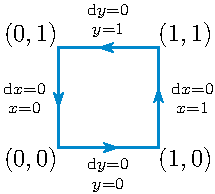
\includegraphics{square.pdf}
\end{center}
So
\begin{align*}
\int_\cC x^2y^2\,\dee{x}+x^3y\,\dee{y} 
&=\int_0^1 x^2\times 0^2\,\dee{x} +\int_0^1 1^3\times y\,\dee{y}
+\int_1^0 x^2\times 1^2\,\dee{x} +\int_1^0 0^3\times y\,\dee{y} \\
&=\frac{1}{2}-\frac{1}{3}
=\frac{1}{6}
\end{align*}

\end{solution}


\begin{question}
For each of the following fields, decide which of the following holds:
\begin{enumerate}[A.]
\item The characterization of conservative vector fields, Theorem~\eref{CLP317}{thm:screenConserv} (with Theorem~\eref{CLP317}{thm:screen}),  tells us $\vF$ is conservative.
\item The characterization of conservative vector fields, Theorem~\eref{CLP317}{thm:screenConserv} (with Theorem~\eref{CLP317}{thm:screen}), tells us $\vF$ is \textbf{not} conservative.
\item The characterization of conservative vector fields, Theorem~\eref{CLP317}{thm:screenConserv} (with Theorem~\eref{CLP317}{thm:screen}), does not tell us whether $\vF$ is conservative or not.
\end{enumerate}
%(The screening test is Theorem~\eref{CLP317}{thm:screen} in the text.)

\begin{enumerate}[a.]
\item $\vF=x\hi + z\hj + y\hk$
\item $\vF=y^2z\hi + x^2z\hj + x^2y\hk$
\item $\vF=(ye^{xy}+1)\hi + (xe^{xy}+z)\hj + \left( \frac1z+y\right)\hk$
\item $\vF=y\cos(xy)\hi + x\sin(xy)\hj $
\end{enumerate}
\end{question}
\begin{hint}
Contrast Theorems~\eref{CLP317}{thm:screenConserv} and \eref{CLP317}{thm:screen}.
\end{hint}
\begin{answer}
a.  A\qquad
b.  B \qquad
c.  A \qquad
d.  B
\end{answer}
\begin{solution}
Every $\vF$ in this problem is defined and has continuous first-order partial derivatives on all of $\mathbb R^2$ or $\mathbb R^3$. The characterization in Theorem~\eref{CLP317}{thm:screenConserv} tells us that our fields will be conservative if and only if they pass the screening test, i.e. have curl 0.

\begin{enumerate}[a.]
\item \begin{align*}\vF&=x\hi + z\hj + y\hk\\
\vnabla \times \vF&=\Big(\frac{\partial F_3}{\partial y} -\frac{\partial F_2}{\partial z} \Big)\hi
+\Big(\frac{\partial F_1}{\partial z} -\frac{\partial F_3}{\partial x} \Big)\hj
+\Big(\frac{\partial F_2}{\partial x} -\frac{\partial F_1}{\partial y} \Big)\hk\\
&=(1-1)\hi+(0-0)\hj+(0-0)\hk = \mathbf0
\end{align*}
This field passes the screening test.  Since $\vF$ is defined and has continuous first-order partial derivatives on all of $\mathbb R^3$, it is conservative. So, we have option A.

\item  \begin{align*}\vF&=y^2z\hi + x^2z\hj + x^2y\hk\\
\vnabla \times \vF&=\Big(\frac{\partial F_3}{\partial y} -\frac{\partial F_2}{\partial z} \Big)\hi
+\Big(\frac{\partial F_1}{\partial z} -\frac{\partial F_3}{\partial x} \Big)\hj
+\Big(\frac{\partial F_2}{\partial x} -\frac{\partial F_1}{\partial y} \Big)\hk\\
&=(x^2-x^2)\hi+(y^2-2xy)\hj+(2xz-2yz)\hk \neq \mathbf0
\end{align*}
So, $\vF$ fails the screening test.  So, it's not conservative. That's option B.

\item 
 \begin{align*}\vF&=(xe^{xy}+1)\hi + (ye^{xy}+z)\hj + \left( \frac1z+y\right)\hk\\
\vnabla \times \vF&=\Big(\frac{\partial F_3}{\partial y} -\frac{\partial F_2}{\partial z} \Big)\hi
+\Big(\frac{\partial F_1}{\partial z} -\frac{\partial F_3}{\partial x} \Big)\hj
+\Big(\frac{\partial F_2}{\partial x} -\frac{\partial F_1}{\partial y} \Big)\hk\\
&=(1-1)\hi+(0-0)\hj+(e^{xy}(xy+1)-xye^{xy}(xy+1))\hk = \mathbf0
\end{align*}
$\vF$ passes the screening test. Since $\vF$ is defined and has continuous first-order partial derivatives on all of $\mathbb R^3$, it is conservative. So, we have option A.

\item
 \begin{align*}\vF&=y\cos(xy)\hi + x\sin(xy)\hj \\
\frac{\partial F_2}{\partial x}&=xy\cos(xy)+\sin(xy)\\
\frac{\partial F_1}{\partial y}&=-xy\sin(xy)+\cos(xy)\\
\frac{\partial F_2}{\partial x}&\neq \frac{\partial F_1}{\partial y}
\end{align*}
$\vF$ fails the screening test, so it is not conservative.
That is Option B.

\end{enumerate}
\end{solution}

%%%%%%%%%%%%%%%%%%%%%%%%%%%%%%%%%%%%%
%%%%%%%%%%%%%%%%%%%
\begin{question}
Let $\varphi(x,y,z)=e^{x^2+y^2}+\cos(z^2)$, and define $\vF = \vnabla \varphi$. Evaluate $\int_C\vF\cdot\dee{\vr}$ over the closed curve $C$ that is an ellipse  traversed clockwise, centred at $(1,2,3)$, passing through the points $(\sqrt5-1,-2,\sqrt5-3)$, $((\sqrt5-2)/2,-1/2,(\sqrt5-6)/2)$, and $(-2,\sqrt 3-2,\sqrt3-3)$.
%%ellipse: r(t)=sqrt5cost-1, sqrt3 sin t -2,x+y-3
\end{question}
\begin{hint}
Please don't do any computation, especially not to find $C$!
\end{hint}
\begin{answer}
0
\end{answer}
\begin{solution}
Since $\vF$ is conservative, $\int_C\vF\cdot\dee{\vr}=0$ over any closed curve $C$. The given curve is closed, so the integral is simply zero.
\end{solution}
%%%%%%%%%%%%%%%%%%%%%%%%%%%%%%%%%%%%%
%%%%%%%%%%%%%%%%%%%
\begin{question}
Let $P_1$ and $P_2$ be points in $\mathbb R^2$. Let $A$ and $B$ be paths from $P_1$ to $P_2$, as shown below.


\begin{center}
\begin{tikzpicture}
\draw[ultra thick, blue] plot[smooth, domain=-.79:3.93]({2*sin( \x r)},{2*sin( (\x*2) r)});
\draw[ultra thick, blue,->] plot[smooth, domain=-.45:-.5]({2*sin( \x r)},{2*sin( (\x*2) r)});
\draw[ultra thick, blue,->] plot[smooth, domain=3.5:3.45]({2*sin( \x r)},{2*sin( (\x*2) r)});
\draw[ultra thick, blue,->] plot[smooth, domain=1.6:1.55]({2*sin( \x r)},{2*sin( (\x*2) r)});
\draw[blue] (2.5,0) node{B};
%\draw (0,0) node[vertex](a){};
\draw (-1.4,2) node[vertex, label=above:${P_1}$](b){};
\draw (-1.4,-2) node[vertex, label=below:${P_2}$](c){};
\draw[ultra thick, red] (b) to[out=224, in=135] (c);
\draw[red] (-2.25,0) node[left]{A};
\draw[ultra thick, red,->] (-2.1,1)--(-2.15,.9);
\end{tikzpicture}
\end{center}

Suppose $\vF$ is a conservative vector field in $\mathbb R^2$ with $\int_A \vF\cdot\dee{\vr}=5$. What is $\int_B \vF\cdot\dee{\vr}?$
\end{question}
\begin{hint}
Review properties of conservative vector fields.
\end{hint}
\begin{answer}
5
\end{answer}
\begin{solution}
Since $\vF$ is conservative, and $A$ and $B$ start and end at the same points, by path-independence 
$\int_B \vF\cdot\dee{\vr}=\int_A \vF\cdot\dee{\vr}=5.$
\end{solution}

%%%%%%%%%%%%%%%%%%%%%%%%%%%%%%%
\begin{question}[M317 2016D] %3
Let $\vF(x, y, z) = e^x \sin y\,\hi + \big[ ae^x \cos y + bz\big]\,\hj 
   + cx\, \hk$. For which values of the constants $a$, $b$, $c$
is $\int_C\vF\cdot\dee{\vr}=0$ for all closed paths $C$?
\end{question}

\begin{hint} 
Review Theorem~\eref{CLP317}{thm:pathIndepConserv} in the text.
\end{hint}

\begin{answer} 
$a=1$, $b=c=0$
\end{answer}

\begin{solution} 
By Theorem~\eref{CLP317}{thm:pathIndepConserv}, the condition that 
 ``$\int_C\vF\cdot\dee{\vr}=0$ for all closed paths $C$''
is equivalent to the condition that ``$\vF$ is conservative'', which, 
since $\vF$ is defined on all of $\bbbr^3$, is equivalent to the condition 
that $\vF$ pass the screening test
\begin{align*}
\vZero =\vnabla\times \vF
&=\det\left[\begin{matrix}\hi&\hj&\hk\\[0.03in] 
     \frac{\partial\hfill}{\partial x}&
        \frac{\partial\hfill}{\partial y}&
        \frac{\partial\hfill}{\partial z}\\[0.03in]
e^x \sin y & ae^x \cos y + bz & cx\end{matrix}\right]
= -b\,\hi-c\,\hj+\big(ae^x\cos y-e^x\cos y\big)\,\hk
\end{align*}
which is the case if and only if $b=c=0$ and $a=1$.
\end{solution}


%%%%%%%%%%%%%%%%%%%%%%%%%%%%%%%
\begin{question}
Consider the four vector fields sketched below. Exactly one of
those vector fields is conservative. Determine which three vector fields 
are not conservative and explain why.
\begin{center}
      (a) \raisebox{-1.0\height}{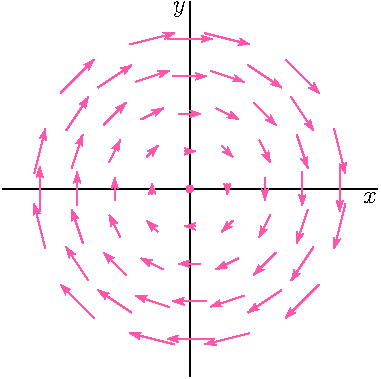
\includegraphics{VFa.pdf}}\qquad
      (b) \raisebox{-1.0\height}{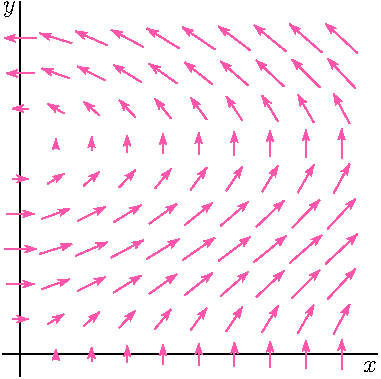
\includegraphics{VFb.pdf}}\qquad
\end{center}
\begin{center}
      (c) \raisebox{-1.0\height}{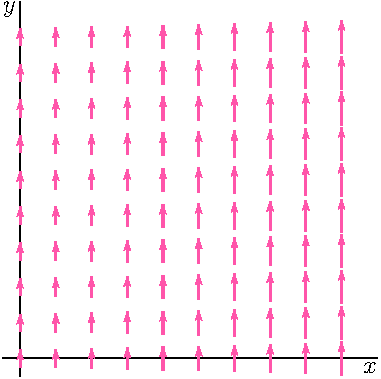
\includegraphics{VFc.pdf}}\qquad
      (d) \raisebox{-1.0\height}{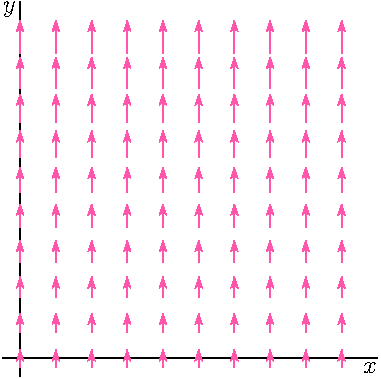
\includegraphics{VFd.pdf}}\qquad
\end{center}
\end{question}

\begin{hint} 
Review Theorem~\eref{CLP317}{thm:pathIndepConserv} in the text.
\end{hint}

\begin{answer} 
(a) Not conservative \quad
(b) Not conservative \quad
(c) Not conservative \quad
(d) Conservative 
\end{answer}

\begin{solution} 
(a) Consider the circle $\cC$ in the figure (a) on the left below,
oriented {\it clockwise}. The vector field $\vF$ is in the same
direction as $\diff{\vr}{t}$ at every point of the curve. 
So $\vF\cdot\diff{\vr}{t}>0$ at every point of $\cC$ and
$\cC$ is a closed curve with $\oint_{\cC}\vF\cdot \dee{\vr}>0$.
As a consequence  $\vF$ is not conservative. 
\begin{center}
      (a) \raisebox{-1.0\height}{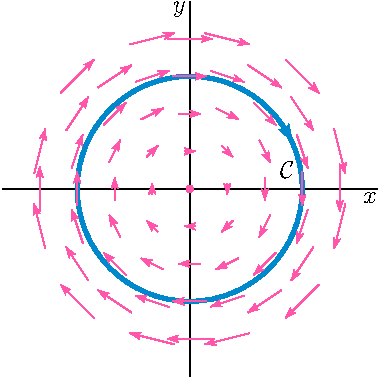
\includegraphics{VFas.pdf}}\qquad
      (b) \raisebox{-1.0\height}{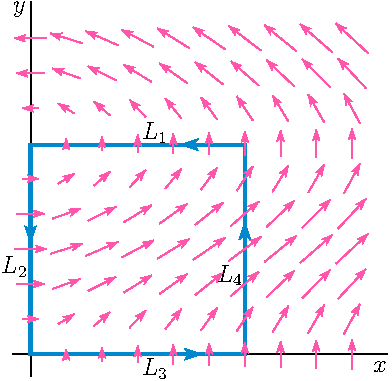
\includegraphics{VFbs.pdf}}\qquad
\end{center}
\smallskip
(b) Consider the square in the figure (b) on the right above,
oriented {\it counterclockwise}. It consists of the four line
segments $L_1$, $L_2$, $L_3$ and $L_4$. On all of $L_1$, $L_2$, $L_3$
we have that $\vF\big(\vr(t)\big)\cdot\vr'(t)=0$ because the vector
field is perpendicular to the line segment. On  $L_4$
we have $\vF\big(\vr(t)\big)\cdot\vr'(t)>0$. So
\begin{align*}
\oint_{\cC}\vF\cdot \dee{\vr} &= \int_{L_1}\vF\cdot \dee{\vr}
                         +\int_{L_2}\vF\cdot \dee{\vr}
                         +\int_{L_3}\vF\cdot \dee{\vr}
                         +\int_{L_4}\vF\cdot \dee{\vr} \\
                         & =0+0+0+\int_{L_4}\vF\cdot \dee{\vr}>0
\end{align*}
So $\cC$ is a closed curve with $\oint_{\cC}\vF\cdot \dee{\vr}>0$
and  $\vF$ is not conservative.


(c) Consider the square in the figure (c) on the left below,
oriented {\it counterclockwise}. It consists of the four line
segments $L_1$, $L_2$, $L_3$ and $L_4$. On $L_1$ and $L_3$
we have that the dot product $\vF\big(\vr(t)\big)\cdot\vr'(t)=0$ because the vector
field is perpendicular to the line segment. On  $L_2$
we have $\vF\big(\vr(t)\big)\cdot\vr'(t)<0$ while on  $L_4$
we have $\vF\big(\vr(t)\big)\cdot\vr'(t)>0$. The vector field
$\vF$ is longer on $L_4$ than on $L_2$. So 
$\vF\big(\vr(t)\big)\cdot\vr'(t)$ has a larger magnitude on $L_4$
than $L_2$ and
\begin{align*}
\oint_{\cC}\vF\cdot \dee{\vr} &= \int_{L_1}\vF\cdot \dee{\vr}
                         +\int_{L_2}\vF\cdot \dee{\vr}
                         +\int_{L_3}\vF\cdot \dee{\vr}
                         +\int_{L_4}\vF\cdot \dee{\vr} \\
                         & =0+\int_{L_2}\vF\cdot \dee{\vr}+0
                           +\int_{L_4}\vF\cdot \dee{\vr}>0
\end{align*}
So $\cC$ is a closed curve with $\oint_{\cC}\vF\cdot \dee{\vr}>0$
and  $\vF$ is not conservative.

\begin{center}
      (c) \raisebox{-1.0\height}{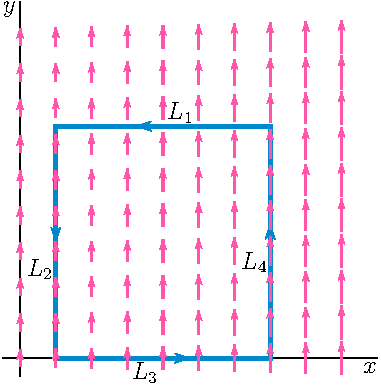
\includegraphics{VFcs.pdf}}\qquad
      (d) \raisebox{-1.0\height}{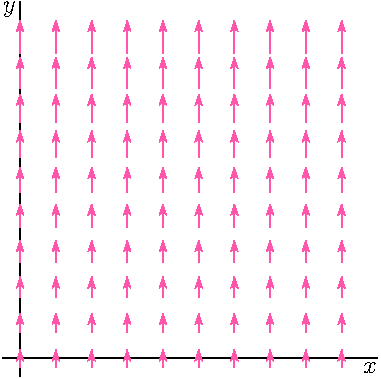
\includegraphics{VFd.pdf}}\qquad
\end{center}


(d) We are told that one of the four vector fields is
conservative. Only the vector field in (d) is left, so it is
conservative. 

\emph{Remark:}
We can verify that vector field (d) is indeed conservative 
by observing (look at the figure (d) on the right above)
that the $\hi$ component of the vector field is exactly 
zero and that the $\hj$  component depends only on $y$. So the 
vector field is of the form 
\begin{equation*}
\vF(x,y) = a(y)\,\hj
\end{equation*}
for some function $a(y)$.
If $A(y)$ is any antiderivative of $a(y)$, we have $\vF=\vnabla A$,
so that $\vF$ is conservative with potential $A(y)$.
\end{solution}


%%%%%%%%%%%%%%%%%%%%%%%%%%
\begin{question}[M317 2007A] %7
Consider the vector field
\begin{equation*}
\vF(x, y, z) = \frac{x-2y}{x^2+y^2}\,\hi
              +\frac{2x + y}{x^2+y^2}\,\hj
              + z\,\hk
\end{equation*}
\begin{enumerate}[(a)]
\item
Determine the domain of $\vF$.
\item
Compute $\vnabla \times \vF$. Simplify the result.
\item
Evaluate the line integral
\begin{equation*}
\int_C \vF \cdot \dee{\vr}
\end{equation*}
where $C$ is the circle of radius $2$ in the plane $z = 3$, 
centered at $(0, 0, 3)$ and traversed counter-clockwise if 
viewed from the positive $z$-axis, i.e. viewed ``from above''.
\item
Is $\vF$ conservative?
\end{enumerate}
\end{question}

\begin{hint} 
Part (d) is a hint.
\end{hint}

\begin{answer} 
(a) The (largest possible) domain is $D=\Set{(x,y,z)}{x^2+y^2\ne 0}$.

(b) $\vnabla\times\vF=\vZero$ on $D$\qquad
(c) $\int_C \vF \cdot \dee{\vr}=4\pi$\qquad
(d) $\vF$ is \emph{not} conservative.
\end{answer}

\begin{solution} 

 (a) The (largest possible) domain is
$
D=\Set{(x,y,z)}{x^2+y^2\ne 0}
$. That is, all of $\mathbb R^3$ except the points lying along the $z$-axis.

\noindent (b) 
As preliminary computations, let's find
\begin{align*}
%\frac{\partial\hfill}{\partial x}\left(\frac{x-2y}{x^2+y^2}\right)
%&=\frac{1}{x^2+y^2}-\frac{2x(x-2y)}{{(x^2+y^2)}^2}
%=\frac{-x^2+y^2+4xy}{{(x^2+y^2)}^2}
%\\
\frac{\partial\hfill}{\partial y}\left(\frac{x-2y}{x^2+y^2}\right)
&=\frac{-2}{x^2+y^2}-\frac{2y(x-2y)}{{(x^2+y^2)}^2}
=\frac{-2x^2+2y^2-2xy}{{(x^2+y^2)}^2}
\\
\frac{\partial\hfill}{\partial x}\left(\frac{2x+y}{x^2+y^2}\right)
&=\frac{2}{x^2+y^2}-\frac{2x(2x+y)}{{(x^2+y^2)}^2}
=\frac{-2x^2+2y^2-2xy}{{(x^2+y^2)}^2}
%\\
%\frac{\partial\hfill}{\partial y}\left(\frac{2x+y}{x^2+y^2}\right)
%&=\frac{1}{x^2+y^2}-\frac{2y(2x+y)}{{(x^2+y^2)}^2}
%=\frac{x^2-y^2-4xy}{{(x^2+y^2)}^2}
\end{align*}
So the curl of $\vF$ is
\begin{align*}
\vnabla\times\vF
&=\det\left[\begin{matrix}
\hi &\hj &\hk \\
\pdiff{}{x} & \pdiff{}{y} & 
                \pdiff{}{z} \\
\frac{x-2y}{x^2+y^2} & \frac{2x + y}{x^2+y^2} & z
\end{matrix}
\right]
=\left(\frac{-2x^2+2y^2-2xy}{{(x^2+y^2)}^2}
  -\frac{-2x^2+2y^2-2xy}{{(x^2+y^2)}^2}\right)\hk
=\vZero
\end{align*}
\emph{on the domain of $\vF$}.

\noindent (c) Parametrize the circle by
\begin{equation*}
\vr(t) = 2\cos t\,\hi +2\sin t\,\hj +3\,\hk\qquad
\vr'(t) = -2\sin t\,\hi +2\cos t\,\hj 
\end{equation*}
with $0\le\theta\le 2\pi$. So the integral is
\begin{align*}
\int_C \vF \cdot \dee{\vr}
&=\int_0^{2\pi}\!\!\bigg\{
       \overbrace{\frac{2\cos t-4\sin t}{4}}^{\frac{x-2y}{x^2+y^2}}\,\hi
      +\overbrace{\frac{4\cos t + 2\sin t}{4}}^{\frac{2x+y}{x^2+y^2}}\,\hj
      + \overbrace{3}^{z}\,\hk\bigg\}
           \cdot
  \Big\{\overbrace{-2\sin t\,\hi +2\cos t\,\hj}^{\vr'(t)}\Big\}\dee{t} \\
&=\int_0^{2\pi}
       \frac{-4\sin t\cos t+8\sin^2 t+8\cos^2t+4\sin t\cos t}{4}\,\dee{t} \\
&= 2\int_0^{2\pi}\dee{t}
=4\pi
\end{align*}

\noindent (d) As the integral of $\vF$ around the simple closed curve $C$
is not zero, $\vF$ cannot be conservative.
See Theorem \eref{CLP317}{thm:pathIndepConserv} and
Examples \eref{CLP317}{eg:screeningCounterexample} and \eref{CLP317}{eg:greenCC}
in the CLP-4  text. 
\end{solution}
%%%%%%%%%%%%%%%%%%%%%%%%%%%%%%%%%%%%%

%%%%%%%%%%%%%%%%%%%
\begin{question}
Find the work, $\int_\cC\vF\cdot \dee{\vr}$, done by the force field 
$\vF=(x+y)\hi+(x-z)\hj+(z-y)\hk$ in moving an object
from $(1,0,-1)$ to $(0,-2,3)$. Does the work done depend on the path used
to get from $(1,0,-1)$ to $(0,-2,3)$?
\end{question}

\begin{hint}
The last part of the question is a huge hint.
\end{hint}

\begin{answer}
$9\frac{1}{2}$ for all paths from $(1,0,-1)$ to $(0,-2,3)$
\end{answer}

\begin{solution}
The point here is that $\vF$ is conservative, as
$\vF=\nabla\phi$ with 
\begin{equation*}
\phi=\frac{x^2}{2}+yx-yz+\frac{z^2}{2}
\end{equation*}
So, for all paths from $\vr(t_0)=(1,0,-1)$ to $\vr(t_1)=(0,-2,3)$,
\begin{align*}
\int_\cC\vF\cdot \dee{\vr}
=\phi\big(\vr(t_1)\big)-\phi\big(\vr(t_0)\big)
&=\phi(0, -2, 3)-\phi(1,0,-1) \\
&=\left[0+0+6+\frac{9}{2}\right]-\left[\frac{1}{2}+0-0+\frac{1}{2}\right] \\
&=9\frac{1}{2}
\end{align*}
.

\end{solution}


%%%%%%%%%%%%%%%%%%
\subsection*{\Procedural}
%%%%%%%%%%%%%%%%%%

%%%%%%%%%%%%%%%%%%%%%%%%%%%%%%%%%%%
\begin{question}
Consider the vector field 
\begin{equation*}
\vV(x, y) = (e^x \cos y + x^2, x^2y + 3)
\end{equation*}
Evaluate the line integral $\int_C\vV\cdot \dee{\vr}$ along the 
oriented  curve $C$ obtained by moving from $(0, 0)$ to $(1,0)$ to 
$(1, \pi)$ and finally to $(0, \pi)$ along straight line segments. 
\end{question}

%\begin{hint} 
%\end{hint}

\begin{answer} 
$2(e-1)+\frac{\pi^2}{2}+3\pi$
\end{answer}

\begin{solution}
Note that:
\begin{itemize}\itemsep1pt \parskip0pt \parsep0pt %\itemindent-15pt
\item
Along the line segment from $(0, 0)$ to $(1,0)$, $x$ increases
from $0$ to $1$, while $y$ is held fixed at $y=0$.
So we may parametrize this segment by $\vr(x) = x\,\hi$, $0\le x\le 1$.
\item
Along the line segment from $(1, 0)$ to $(1,\pi)$, $y$ increases
from $0$ to $\pi$, while $x$ is held fixed at $x=1$.
So we may parametrize this segment by $\vr(x) = \hi + y\,\hj$, $0\le y\le\pi$.
\item
Along the line segment from $(1, \pi)$ to $(0,\pi)$, $x$ decreases
from $1$ to $0$, while $y$ is held fixed at $y=\pi$.
So we may parametrize this segment by $\vr(x) = x\,\hi+\pi\,\hj$
with $x$ running from $1$ to $0$.
\end{itemize}
Hence
\begin{align*}
\int_C \vV\cdot \dee{\vr}
&=\int_0^1 \vV(x,0)\cdot\hi\ \dee{x}+\int_0^\pi \vV(1,y)\cdot\hj\ \dee{y}
+\int_1^0 \vV(x,\pi)\cdot\hi\ \dee{x}\\
&=\int_0^1 (e^x+x^2)\ \dee{x}
         +\int_0^\pi (y+3)\ \dee{y}+\int_1^0 (-e^x+x^2)\ \dee{x}\cr
&=2\int_0^1 e^x\ \dee{x}+\int_0^\pi (y+3)\ \dee{y}\\
&=2(e-1)+\frac{\pi^2}{2}+3\pi
\end{align*}
\end{solution}


%%%%%%%%%%%%%%%%%%%
\begin{question}
Evaluate $\int_\cC\vF\cdot \dee{\vr}$ for 
\begin{enumerate}[(a)]
\item 
$\vF(x,y)=xy\,\hi-x^2\,\hj$ along $y=x^2$ from $(0,0)$ to $(1,1)$.

\item
$\vF(x,y,z)=(x-z)\,\hi+(y-z)\,\hj-(x+y)\,\hk$ along the polygonal path from
$(0,0,0)$ to $(1,0,0)$ to $(1,1,0)$ to $(1,1,1)$.	
\end{enumerate}
\end{question}

%\begin{hint}
%\end{hint}

\begin{answer}
(a) $-\frac{1}{4}$ \qquad
(b) $-1$	
\end{answer}

\begin{solution}
(a) 
We may parametrize the curve by $\vr(t)=t\,\hi+t^2\,\hj$ with $0\le t\le 1$.
Then $\vv(t)=\diff{\vr}{t}(t)=\hi+2t\,\hj$ and 
$\vF\big(x(t),y(t)\big)=t^3\,\hi-t^2\,\hj$ so
\begin{align*}
\int_\cC\vF\cdot \dee{\vr}
&=\int_0^1 \vF\big(x(t),y(t)\big)\cdot \diff{\vr}{t}(t)\ \dee{t}
=\int_0^1\big[t^3\,\hi-t^2\,\hj\big]
\cdot\big[\hi+2t\,\hj\big]\,\dee{t}
=\int_0^1\big[-t^3\big]\,\dee{t} \\
&=-\frac{1}{4}
\end{align*}

(b) The path is the union of three line segments.
\begin{itemize}\itemsep1pt \parskip0pt \parsep0pt %\itemindent-15pt
\item
On the first segment of the path $y=z=0$ so $\vF$ simplifies
to $x\,\hi-x\,\hk$ and $\dee{\vr}=\hi\ \dee{x}$ (i.e. we can parametrize
the first segment of the path by $\vr(x)=x\,\hi$ with $0\le x\le 1$),
so $\vF\cdot \dee{\vr}=x\,\dee{x}$. 
\item
On the second segment of the path $x=1$, $z=0$ so $\vF$ simplifies
to $\hi+y\hj-(1+y)\hk$ and $\dee{\vr}=\hj\, \dee{y}$
(parametrize the second segment of the path by $
\vr(y)=\hi+y\,\hj$ with $0\le y\le 1$),
so $\vF\cdot \dee{\vr}=y\,\dee{y}$.
\item
On the final segment of the path $x=y=1$ so $\vF$ simplifies
to $(1-z)\hi+(1-z)\hj-2\hk$ and $\dee{\vr}=\hk\, \dee{z}$
(parametrize the third segment of the path by $
\vr(z)=\hi+\hj+z\,\hk$ with $0\le z\le 1$),
so $\vF\cdot \dee{\vr}=-2\,\dee{z}$.
\end{itemize}
So
\begin{equation*}
\int_\cC\vF\cdot \dee{\vr}=\int_0^1 x\,\dee{x}
           +\int_0^1 y\,\dee{y}+\int_0^1(-2)\,\dee{z}
=\frac{1}{2}+\frac{1}{2}-2
=-1
\end{equation*}
\end{solution}

%%%%%%%%%%%%%%%%%%%%%%%%%%%
\begin{question}[M317 1998D] %2
Let $\cC$ be the part of the curve of intersection of $xyz=8$
and $x=2y$ which lies between the points $(2,1,4)$ and $(4,2,1)$. Calculate
$$
\int_\cC \vF\cdot \dee{\vr}
$$
where
$$
\vF = x^2\,\hi+(x-2y)\,\hj+x^2 y\,\hk
$$
\end{question}

\begin{hint} 
Parametrize the curve using $y$ as a parameter. 
\end{hint}

\begin{answer}
$-\frac{40}{3}$
\end{answer}

\begin{solution} 
Parametrize the curve using $y$ as a parameter. Then $y=t$, $x=2y=2t$ and 
$z=\frac{8}{xy}=\frac{8}{2t^2}$ so that:
\begin{align*}
\vr(t)&=2t\,\hi+t\,\hj+\frac{4}{t^2}\,\hk,\qquad 1\le t\le 2\\
\vr'(t)&=2\,\hi+\hj-\frac{8}{t^3}\,\hk\\
\vF(\vr(t))&= 4t^2\,\hi+4t^3\,\hk\\
\vF(\vr(t))\cdot \vr'(t)&=8t^2-32
\end{align*}
Then
$$
\int_\cC \vF\cdot \dee{\vr}
=\int_1^2 \vF(\vr(t))\cdot \vr'(t)\ \dee{t}
=\int_1^2 \big(8t^2-32\big)\ \dee{t}
= \left[\frac{8}{3}t^3-32t\right]_1^2
=-\frac{40}{3}
$$

\end{solution}


%%%%%%%%%%%%%%%%%%%%%%%%%%%
\begin{question}[M317 2003A] %2
Let $\ \vF= e^x\sin y\,\hi+[ae^x\cos y+bz]\,\hj+cx\,\hk$. 
For which values of the constants $a,\ b,\ c$ is 
$\ \int_C\vF\cdot \dee{\vr}=0\ $ for all closed paths $C$?
\end{question}

\begin{hint} 
Use Theorems~\eref{CLP317}{thm:pathIndepConserv} and \eref{CLP317}{thm:screenConserv} in the CLP-4 text.
\end{hint}

\begin{answer} 
$a=1,\ b=c=0$
\end{answer}

\begin{solution} 
Note $\vF$ is defined and continuous on all of $\mathbb R^3$. By  Theorem~\eref{CLP317}{thm:pathIndepConserv}, the integral $\ \int_C\vF\cdot \dee{\vr}=0\ $ for all closed paths $C$
if and only if $\vF$ is conservative. Furthermore, $\vF$ has continuous first-order partial derivatives on all of $\bbbr^3$. Using Theorem~\eref{CLP317}{thm:screenConserv}, $\vF$ is conservative if
and only if $\vnabla\times\vF=\vZero$:
\begin{align*}
\vZero=\vnabla\times\vF
&=\det\left[\begin{matrix}\hi&\hj&\hk\\[0.03in] 
            \frac{\partial\hfill}{\partial x}&
            \frac{\partial\hfill}{\partial y}&
            \frac{\partial\hfill}{\partial z}\\[0.03in]
  e^x\sin y & ae^x\cos y+bz & cx\end{matrix}\right] \\
&=(0-b)\hi-(c-0)\hj+(ae^x\cos y-e^x\cos y)\hk
\end{align*}
So $a=1,\ b=c=0$.
\end{solution}

%%%%%%%%%%%%%%%%%%%%%%%%%%%%%%%%%%%
\begin{question}
 Let  $\vF = 6x^2yz^2\,\hi + (2x^3z^2 + 2y - xz)\,\hj 
+ 4x^3yz\,\hk$ and let $\vG = yz\,\hi + xy\,\hk$. 
\begin{enumerate}[(a)]
\item 
For what value of the constant $\la$ is the vector field 
$\vH = \vF +  \la\vG$ conservative on 3-space? 
\item
Find a scalar potential $\phi(x,y,z)$ for the conservative field $\vH$ referred to in part (a). 
\item 
Find   $\int_C\vF\cdot \dee{\vr}$ if $C$ is the curve of intersection of the two surfaces $z = x$ and $y = e^{xz}$ from the point $(0, 1, 0)$ to 
the point $(1, e, 1)$.
\end{enumerate} 
\end{question}

\begin{hint} 
(a) Use Theorem~\eref{CLP317}{thm:screenConserv} in the CLP-4 text.

(c) You may parametrize the curve using $x$ as the parameter.
Exploit the fact that, for the value of $\la$ found in part (a), $\vF+\la \vG$ is conservative.
\end{hint}

\begin{answer} 
(a) $\la=-1$\qquad
(b) $\phi(x,y,z)=2x^3yz^2-xyz+y^2+K$, for any constant $K$

(c) $e^2+2e-2$
\end{answer}

\begin{solution}
(a), (b) The curls of $\vF$ and $\vG$ are
\begin{align*}
\vnabla\times\vF
&= \det\left[\begin{matrix}
                       \hi &       \hj        &   \hk \\
               \pdiff{}{x} &   \pdiff{}{y}    &  \pdiff{}{z} \\
                  6x^2yz^2 & 2x^3z^2 + 2y - xz &  4x^3yz
            \end{matrix}\right] \\
&=(4x^3z-4x^3z+x)\,\hi-(12x^2yz-12x^2yz)\,\hj+(6x^2z^2-z-6x^2z^2)\,\hk \\
&=x\,\hi-z\,\hk\\
\vnabla\times\vG
&=\det\left[\begin{matrix}
                   \hi       &   \hj       &  \hk \\
                 \pdiff{}{x} & \pdiff{}{y} &  \pdiff{}{z} \\
                          yz &      0      & xy
\end{matrix}\right] \\
&=x\hi-z\,\hk
\end{align*}
Hence the screening test for
\begin{equation*}
\vnabla\times\big(\vF+\la\vG\big)=(x+\la x)\,\hi-(z+\la z)\,\hk
\end{equation*}
passes for $\la=-1$. Furthermore
\begin{align*}
\vF-\vG &=(6x^2yz^2-yz)\,\hi+(2x^3z^2 + 2y - xz)\,\hj+(4x^3yz-xy)\,\hk \\
&=\vnabla\big(2x^3yz^2-xyz+y^2\big)
\end{align*}
The potential was found by guessing. Alternatively,
we can find it by using that
$\phi(x,y,z)$ is a potential for $\vF-\vG$ 
if and only if
\begin{align*}
\pdiff{\phi}{x}(x,y,z) &= 6x^2yz^2-yz \\
\pdiff{\phi}{y}(x,y,z) &= 2x^3z^2 + 2y - xz \\
\pdiff{\phi}{z}(x,y,z) &= 4x^3yz-xy
\end{align*}
Integrating the first of these equations gives
\begin{equation*}
\phi(x,y,z) = 2x^3yz^2-xyz + f(y,z)
\end{equation*}
Substituting this into the second equation gives 
\begin{equation*}
2x^3z^2-xz + \pdiff{f}{y}(y,z) 
   = 2x^3z^2 + 2y - xz \qquad\hbox{or}\qquad 
\pdiff{f}{y}(y,z) = 2y
\end{equation*}
which integrates to
\begin{equation*}
f(y,z) = y^2+ g(z)
\end{equation*}
Finally, substituting $\phi(x,y,z) = 2x^3yz^2-xyz + y^2 + g(z)$
into the last equation gives
\begin{equation*}
4x^3yz-xy + g'(z) = 4x^3yz-xy\qquad\hbox{or}\qquad 
g'(z) = 0
\end{equation*}
which integrates to
\begin{equation*}
g(z) =  K
\end{equation*}
with $K$ being an arbitrary constant.
Choosing $K=0$ gives the potential $\phi(x,y,z) =  2x^3yz^2-xyz + y^2$
as in the guess above.


(c) Any point $(x,y,z)$ on the curve must have $z=x$ and $y=e^{xz}=e^{x^2}$.
So we may parametrize the curve by
$\vr(x)=x\,\hi+e^{x^2}\,\hj+x\,\hk$, $0\le x\le 1$. Hence
\begin{align*}
\int_C\vF\cdot \dee{\vr}
&=\int_C(\vF-\vG)\cdot \dee{\vr}+\int_C\vG\cdot \dee{\vr}\\[-0.2in]
&=\Big[2x^3yz^2-xyz+y^2\Big]_{(0,1,0)}^{(1,e,1)}
+\int_0^1\overbrace{[xe^{x^2}\hi + xe^{x^2}\hk]}^{\vG(\vr(x))}\cdot 
   \overbrace{[\hi+2xe^{x^2}\,\hj+\hk]}^{\diff{\vr}{x}}\ \dee{x}\\
&=e+e^2-1+\int_0^1 2xe^{x^2}\ \dee{x}
=e+e^2-1+\Big[e^{x^2}\Big]_0^1
=e^2+2e-2
\end{align*}
\end{solution}

%%%%%%%%%%%%%%%%%%%%%%%%%%%%%%%
\begin{question}[M317 2016D] %6
Find the work done by the force field 
$\vF(x,y,z) = (x - y^2\,,\, y - z^2\,,\, z - x^2)$ on a particle 
that moves along the line segment from $(0, 0, 1)$ to $(2, 1, 0)$.
\end{question}

%\begin{hint} 
%
%\end{hint}

\begin{answer} 
$\frac{7}{3}$
\end{answer}

\begin{solution} 
Parametrize the line segment by
\begin{equation*}
\vr(t) = (0,0,1) + t\big\{(2,1,0)-(0,0,1)\big\}
       = \big(2t,t,1-t\big)\qquad
0\le t\le 1
\end{equation*}
so that $\vr(0) = (0,0,1)$ is the initial point of the line segment and
$\vr(1) = (2,1,0)$ is the final point of the segment. Then
\begin{equation*}
\vr'(t) = (2,1,-1)\qquad
% \diff{s}{t}(t) = |\vr'(t)| = \sqrt{6}
\end{equation*}
and the work is
\begin{align*}
\int\vF\cdot\dee{\vr}
&=\int_0^1 \vF\big(\vr(t)\big)\cdot \vr'(t)\,\dee{t}
=\int_0^1\big(2t-t^2\,,\, t-(1-t)^2 \,,\,(1-t)-4t^2\big)\cdot(2,1,-1)\,\dee{t}
\\
&=\int_0^1\big(4t-2t^2 \ +\ t-1+2t-t^2 \ -\ 1+t+4t^2\big)\,\dee{t}
=\int_0^1\big(t^2+8t-2\big)\,\dee{t} \\
&=\frac{1}{3}+4-2
=\frac{7}{3}
\end{align*}
\end{solution}

%%%%%%%%%%%%%%%%%%%%%%%%%%%
\begin{question}[M317 2003A] %3
Let $\ \vF= \frac{x}{x^2+y^2}\,\hi+\frac{y}{x^2+y^2}\,\hj+x^3\,\hk$. 
Let $P$ be the path which starts at $(1,0,0)$, ends at 
$\big(\frac{1}{\sqrt{2}},\frac{1}{\sqrt{2}},\frac{1}{2}\ln 2\big)$ and follows
\begin{equation*}
x^2+y^2=1\qquad xe^z=1
\end{equation*}
Find the work done in moving a particle along $P$ in the field $\vF$.
\end{question}

\begin{hint} 
Parametrize the path using sines and cosines. The work done is $\int_C \vF \cdot \dee{\vr}$
\end{hint}

\begin{answer} 
$\frac{1}{3}\big[1-\frac{1}{2^{3/2}}\big]\approx 0.2155$
\end{answer}

\begin{solution} 
On $P$, $z=\ln\frac{1}{x}=-\ln(x)$. So parametrize the curve 
$P$ by
\begin{equation*}
\vr(\theta)=\cos\theta\,\hi+\sin\theta\,\hj-\ln(\cos\theta)\,\hk\qquad
0\le\theta\le\frac{\pi}{4}
\end{equation*}
Then
\begin{align*}
\vr\,'(\theta)&=-\sin\theta\,\hi+\cos\theta\,\hj+\tan\theta\,\hk\\
\vF\big(\vr(\theta)\big)&=\cos\theta\,\hi+\sin\theta\,\hj+\cos^3\theta\,\hk\\
\vF\big(\vr(\theta)\big)\cdot\vr\,'(\theta)&=\sin\theta\cos^2\theta\\
\end{align*}
so that
\begin{align*}
\text{Work}
&=\int_P\vF\cdot \dee{\vr}
=\int_0^{\pi/4}\vF\big(\vr(\theta)\big)\cdot\vr\,'(\theta)\ \dee{\theta}
=\int_0^{\pi/4}\sin\theta\cos^2\theta\ \dee{\theta}
=-\frac{1}{3}\cos^3\theta\Big|_0^{\pi/4} \\
&=\frac{1}{3}\big[1-\frac{1}{2^{3/2}}\big]\approx 0.2155
\end{align*}
\end{solution}


%%%%%%%%%%%%%%%%%%%%%%%%%%%
\begin{question}[M317 2005A] %2
Let $\vF = \big(yz\cos x\,,\,z\sin x+2yz\,,\,y\sin x+y^2-\sin z\big)$
and let $C$ be the line segment $\vr(t) = (t,t,t)$, for $0\le t\le\pi/2$.
Evaluate $\displaystyle\int_C\vF\cdot\dee{\vr}$.
\end{question}

\begin{hint}
Is $\vF$ conservative? 
\end{hint}

\begin{answer} 
$\frac{\pi^3}{8}+\frac{\pi^2}{4}-1$
\end{answer}

\begin{solution} 
Hmmm. $\vF$ looks suspiciously complicated. Let's
guess that $\vF$ is conservative and look for a potential for it.
$\phi(x,y,z)$ is a potential for this $\vF$ if and only if
\begin{align*}
\frac{\partial \varphi}{\partial x}(x,y,z) &= yz\cos x \\
\frac{\partial \varphi}{\partial y}(x,y,z) &= z\sin x+2yz \\
\frac{\partial \varphi}{\partial z}(x,y,z) &= y\sin x+y^2-\sin z
\end{align*}
Integrating the first of these equations gives
\begin{equation*}
\varphi(x,y,z) = yz\sin x + f(y,z)
\end{equation*}
Substituting this into the second equation gives 
\begin{equation*}
z\sin x + \pdiff{f}{y}(y,z) 
= z\sin x+2yz\qquad\text{or}\quad
\pdiff{f}{y}(y,z) = 2yz
\end{equation*}
which integrates to
\begin{equation*}
f(y,z) = y^2z + g(z)
\end{equation*}
Finally, substituting $\varphi(x,y,z) = yz\sin x+y^2z + g(z)$
into the last equation gives
\begin{equation*}
y\sin x+y^2 + g'(z) 
= y\sin x+y^2-\sin z\qquad\text{or}\quad
g'(z) = -\sin z
\end{equation*}
which integrates to
\begin{equation*}
g(z) = \cos z + C
\end{equation*}
with $C$ being an arbitrary constant.
So $\phi(x,y,z)=yz\sin x+y^2z+\cos z$ is one allowed scalar potential
and the specified integral is
\begin{align*}
\int_C\vF\cdot\dee{\vr} = \varphi(\vr)\Big|_{\vr(0)}^{\vr(\pi/2)}
= \varphi(\pi/2\,,\,\pi/2\,,\,\pi/2) -\varphi (0,0,0)
= \frac{\pi^3}{8}+\frac{\pi^2}{4}-1
\end{align*}

\end{solution}

%%%%%%%%%%%%%%%%%%%%%%%%%%%%%%%

%%%%%%%%%%%%%%%%%%%%%%%%%%%
\begin{question}[M317 2010D]    %2
Let $C$ be the upper half of the unit circle centred on $(1, 0)$ 
(i.e. that part of the circle which lies above the $x$-axis), 
oriented clockwise. Compute the line integral
$\int_C xy\,\dee{y}$.
\end{question}

\begin{hint} 
Is $\vF= xy\,\hj$ conservative? Sketch $C$.
\end{hint}

\begin{answer} 
$-\frac{2}{3}$
\end{answer}

\begin{solution} 
\textbf{Solution 1:}\\
We are being asked to evaluate the line integral 
$\int_C\vF\cdot\dee{\vr}$ with $C$ being the specified semi-circle and 
$\vF=xy\,\hj$. As $\vnabla\times\vF\ne\vZero$, the vector field $\vF$
is not conservative. So we'll evaluate the integral directly. 
First, using the figure,
\begin{center}
       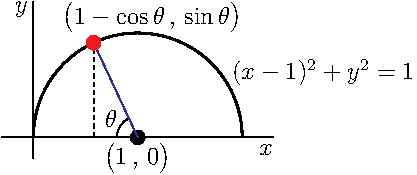
\includegraphics{OE10D_2.pdf}
\end{center}
\noindent
we parametrize $C$ by 
\begin{equation*}
\vr(\theta) = 
\big(x(\theta)\,,\,y(\theta)\big)
=(1-\cos\theta)\,\hi +\sin\theta\,\hj\qquad 0\le\theta\le\pi
\end{equation*}
So the integral is
\begin{align*}
\int_C xy\,\dee{y}
=\int_0^\pi x(\theta)\,y(\theta)\, y'(\theta)\ \dee{\theta}
=\int_0^\pi (1-\cos\theta)\,\sin\theta\,\cos\theta \ \dee{\theta}
\end{align*}
Making the substitution $u=\cos\theta$, $\dee{u} =-\sin\theta\,\dee{\theta}$,
$u(0)=1$, $u(\pi)=-1$,
\begin{align*}
\int_C xy\,\dee{y}
=\int_1^{-1} (1-u)\, u\, (-\dee{u})
=\int_{-1}^1 (u-u^2)\,\dee{u}
=-2 \int_0^1 u^2\,\dee{u}
=-2 \frac{1^3}{3}=-\frac{2}{3}
\end{align*}

\textbf{Solution 2:}\\
We can write $x$ in terms of $y$ over $C$ in two pieces:
\begin{itemize}
\item Let $C_1$ be the quarter-circle $x=1-\sqrt{1-y^2}$ as $y$ goes from 0 to 1,  and
\item Let $C_2$ be the quarter-circle $x=1+\sqrt{1-y^2}$ as $y$ goes from 1 to 0.
\end{itemize}
Then:
\begin{align*}
\int_C xy\dee{y} &=\int_{C_1} xy\dee{y}+\int_{c_2}xy\dee{y}\\
&=\int_0^1\left(1-\sqrt{1-y^2}\right)y\,\dee{y}+\int_1^0\left(1+\sqrt{1-y^2}\right)y\,\dee{y}\\
&=\int_0^1 y\,\dee{y}-\int_0^1y\sqrt{1-y^2}\,\dee{y}+\int_1^0y\,\dee{y}+\int_1^0 y\sqrt{1-y^2}\,\dee{y}\\
&=-2\int_0^1 y\sqrt{1-y^2}\,\dee{y}
\intertext{Using the substitution $u=1-y^2$, $\dee{u}=-2y\,\dee{y}$:}
&=\int_1^0u^{1/2}\dee{u}=-\frac23
\end{align*}
\end{solution}


%%%%%%%%%%%%%%%%%%%%%%%%%%%%
\begin{question}[M317 2006D] %7
Show that the following line integral is independent of path and 
evaluate the integral.
\begin{align*}
\int_C (ye^x + \sin y)\,\dee{x} + (e^x + \sin y + x \cos y)\,\dee{y}
\end{align*}
where $C$ is any path from $(1, 0)$ to $(0, \pi/2)$.
\end{question}

\begin{hint} 
That the line integral is to be independent of path is a huge hint.
\end{hint}

\begin{answer} 
The line integral is independent of path because it is of the form 
$\int_C \vF\cdot\dee{\vr}$ with $\vF$ being a conservative field. The value
of the integral is $1+\frac{\pi}{2}$.
\end{answer}

\begin{solution}

The line integral is $\int_C \vF\cdot\dee{\vr}$ with
$\vF = (ye^x + \sin y)\,\hi + (e^x + \sin y + x \cos y)\,\hj$.
We are to show that it is independent of path. That is the case if and
only if $\vF$ is conservative. So let's look for a potential $\varphi$
for $\vF$. That is, let's look for a function $\varphi$ that obeys
\begin{align*}
\frac{\partial \varphi}{\partial x}(x,y) 
&= ye^x + \sin y \\
\frac{\partial \varphi}{\partial y}(x,y) &= e^x + \sin y + x \cos y 
\end{align*}
Integrating the first of these equations gives
\begin{equation*}
\varphi(x,y) = ye^x + x\sin y + f(y)
\end{equation*}
Substituting this into the second equation gives 
\begin{equation*}
e^x + x\cos y + f'(y) = e^x + \sin y + x \cos y\qquad\text{or}\quad
f'(y) = \sin y
\end{equation*}
which integrates to
\begin{equation*}
f(y) = -\cos y + C
\end{equation*}
So $\vF$ is indeed conservative with one potential being
$\varphi(x,y) = ye^x + x\sin y -\cos y$ and the line integral is
\begin{align*}
\int_C (ye^x + \sin y)\,\dee{x} + (e^x + \sin y + x \cos y)\,\dee{y}
&=\int_C \vF\cdot\dee{\vr}
=\varphi(x,y)\Big|^{(0,\pi/2)}_{(1,0)} \\
&=\Big[ye^x + x\sin y -\cos y\Big]^{(0,\pi/2)}_{(1,0)} \\
&=1+\frac{\pi}{2}
\end{align*}

\end{solution}

%%%%%%%%%%%%%%%%%%%%%%%%%%%%
\begin{question}[M317 2006D] %1
Evaluate the integral
\begin{align*}
\int_C xy \,\dee{x} + yz \,\dee{y} + zx \,\dee{z}
\end{align*}
around the triangle with vertices $(1, 0, 0)$, $(0, 1, 0)$, and $(0, 0, 1)$, 
oriented clockwise as seen from the point $(1, 1, 1)$.
\end{question}

\begin{hint} 
Note that 
\begin{itemize}\itemsep1pt \parskip0pt \parsep0pt %\itemindent-15pt
\item[$\circ$]
$y=0$ on the line segment from $(1,0,0)$ to $(0, 0, 1)$ and
\item[$\circ$]
$x=0$ on the line segment from $(0,0,1)$ to $(0, 1, 0)$ and 
\item[$\circ$]
$z=0$ on the line segment from $(0, 1, 0)$ to $(1, 0, 0)$
\end{itemize}
\end{hint}

\begin{answer} 
$\frac{1}{2}$
\end{answer}

\begin{solution}
Here is a sketch of $C$.

\begin{center}
       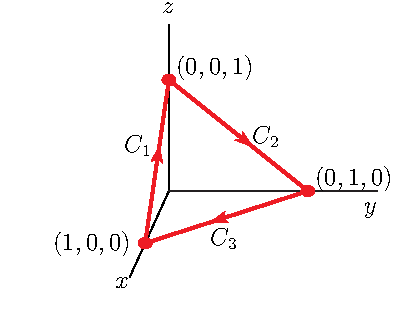
\includegraphics{OE06D_1.pdf}
\end{center}


Note that 
\begin{itemize}\itemsep1pt \parskip0pt \parsep0pt %\itemindent-15pt
\item[$\circ$]
$y=0$ on the line segment from $(1, 0, 0)$ to $(0,0,1)$ so that 
the integral reduces to $\int zx \,\dee{z}$ on that line segment and
\item[$\circ$]
$x=0$ on the line segment from $(0,0,1)$ to $(0, 1, 0)$ so that 
the integral reduces to $\int yz \,\dee{y}$ on that line segment and  
\item[$\circ$]
$z=0$ on the line segment from $(0, 1, 0)$ to  $(1, 0, 0)$ so that 
the integral reduces to $\int xy \,\dee{x}$ on that line segment.
\end{itemize}
So it looks feasible to evaluate the integral directly. 
Label the sides of the triangle $C_1$, $C_2$ and $C_3$ as in the
sketch above.
\begin{itemize}\itemsep1pt \parskip0pt \parsep0pt %\itemindent-15pt
\item[$\circ$]
We parametrize $C_1$ by $\vr(t) = (1,0,0) + t[(0,0,1)-(1,0,0)]
                                = (1-t\,,\,0\,,\,t)$, $0\le t\le 1$.
So
\begin{align*}
\int_{C_1} xy \,\dee{x} + yz \,\dee{y} + zx \,\dee{z}
&= \int_{C_1}  zx \,\dee{z}
=\int_0^1 \overbrace{(1-t)}^{x}
         \overbrace{(t)}^{z}
          \overbrace{(1)}^{z'(t)}\,\dee{t}
=\int_0^1 (t-t^2)\,\dee{t} \\
&=\frac{1}{2}-\frac{1}{3} =\frac{1}{6}
\end{align*}
\item[$\circ$]
We parametrize $C_2$ by $\vr(t) = (0,0,1) + t[(0,1,0)-(0,0,1)]
                                = (0\,,\,t\,,\,1-t)$, $0\le t\le 1$.
So
\begin{align*}
\int_{C_2} xy \,\dee{x} + yz \,\dee{y} + zx \,\dee{z}
&= \int_{C_2}  yz \,\dee{y}
=\int_0^1 \overbrace{(t)}^{y}
         \overbrace{(1-t)}^{z}
          \overbrace{(1)}^{y'(t)}\,\dee{t}
=\int_0^1 (t-t^2)\,\dee{t} \\
&=\frac{1}{2}-\frac{1}{3} =\frac{1}{6}
\end{align*}
\item[$\circ$]
We parametrize $C_3$ by $\vr(t) = (0,1,0) + t[(1,0,0)-(0,1,0)]
                                = (t\,,\,1-t\,,\,0)$, $0\le t\le 1$.
So
\begin{align*}
\int_{C_3} xy \,\dee{x} + yz \,\dee{y} + zx \,\dee{z}
&= \int_{C_3}  xy \,\dee{x}
=\int_0^1 \overbrace{(t)}^{x}
         \overbrace{(1-t)}^{y}
          \overbrace{(1)}^{x'(t)}\,\dee{t}
=\int_0^1 (t-t^2)\,\dee{t} \\
&=\frac{1}{2}-\frac{1}{3} =\frac{1}{6}
\end{align*}
\end{itemize}
All together
\begin{align*}
\int_{C} xy \,\dee{x} + yz \,\dee{y} + zx \,\dee{z}
&=\sum_{\ell=1}^3\int_{C_\ell} xy \,\dee{x} + yz \,\dee{y} + zx \,\dee{z}
=3\times\frac{1}{6}=\frac{1}{2}
\end{align*}
\end{solution}

%%%%%%%%%%%%%%%%%%%%%%%%%%%
\begin{question}[M317 2008D] %5
Evaluate the line integral $\int_C \vF\cdot \dee{\vr}$, where $\vF$  
is the conservative vector field
\begin{equation*}
\vF (x, y, z) = \big(y + ze^x , x + e^y \sin z, z + e^x + e^y \cos z\big)
\end{equation*}
and $C$ is the curve given by the parametrization
\begin{equation*}
\vr(t) = (t, e^t , \sin t),\qquad
\text{$t$ from $0$ to $\pi$} .
\end{equation*}
\end{question}

\begin{hint} 
That $\vF$ is conservative should be a dead giveaway.
\end{hint}

\begin{answer} 
$\pi e^\pi$
\end{answer}

\begin{solution} 
We are told that $\vF$ is conservative. Let's find a potential
$\varphi$ obeying $\vnabla\varphi = \vF$. That is,
\begin{align*}
\frac{\partial\varphi}{\partial x}
   &= y + ze^x \\
\frac{\partial\varphi}{\partial y}
   &= x + e^y \sin z \\
\frac{\partial\varphi}{\partial z}
   &= z + e^x + e^y \cos z 
\end{align*}
The first equation forces $\varphi(x,y,z) = xy +ze^x +\psi(y,z)$.
Substituting this into the second equation gives
$x+\frac{\partial\psi}{\partial y}(y,z) = x + e^y \sin z$ 
or $\frac{\partial\psi}{\partial y}(y,z) = e^y \sin z$
which forces $\psi(y,z) = e^y\sin z +\zeta(z)$. So far, we have
$\varphi(x,y,z) = xy +ze^x +e^y\sin z +\zeta(z)$.
Substituting this into the third equation gives
$e^x +e^y\cos z +\zeta'(z) = z + e^x + e^y \cos z$ or 
$\zeta'(z) = z$ which forces $\zeta(z) = \frac{z^2}{2}+C$, for some constant
$C$, which we take to be zero. So our potential is
\begin{equation*}
\varphi(x,y,z) = xy +ze^x +e^y\sin z +\frac{z^2}{2}
\end{equation*}
So the line integral
\begin{equation*}
\int_C \vF\cdot \dee{\vr}
=\varphi\big(\vr(\pi)\big) -\varphi\big(\vr(0)\big)
=\varphi\big(\pi,e^\pi,0\big) -\varphi\big(0,1,0\big)
=\pi e^\pi
\end{equation*}

\end{solution}



%%%%%%%%%%%%%%%%%%%%%%%%%%%
\begin{question}[M317 2002A] %4
\begin{enumerate}[(a)]
\item  %(a) 
For which values of the constants $\alpha$, $\beta$ and $\gamma$
is the vector field
$$
\vF(x,y,z) = \alpha e^y\,\hi+(xe^y+\beta\cos z)\,\hj-\gamma y\sin z\,\hk
$$
conservative?
\item %(b) 
For those values of $\alpha$,\ $\beta$ and $\gamma$ found in part
(a), calculate $\int_C \vF\cdot \dee{\vr}$, where $C$ is the curve parametrized
by $x=t^2$, $y=e^t$, $z=\pi t$, $0\le t\le 1$.
\end{enumerate}
\end{question}

\begin{hint} 
To calculate the integral, it might be easier to find a potential for $\vF$ and use Theorem~\eref{CLP317}{thm:workIntegral}.
\end{hint}

\begin{answer} 
(a) $\alpha=1$, $\beta=\gamma$\qquad
(b) $e^e-\beta(e+1)$
\end{answer}


\begin{solution}
(a)
Note $\vF$ is defined and continuous on all of $\mathbb R^3$. Furthermore, $\vF$ has continuous first-order partial derivatives on all of $\bbbr^3$. Using Theorem~\eref{CLP317}{thm:screenConserv}, $\vF$ is conservative if
and only if it has zero curl:
% $\vF$ is conservative if and only if
\begin{align*}
0&=\vnabla\times\vF
=\vnabla\times\big(\alpha e^y\,\hi+(xe^y+\beta\cos z)\,\hj
                   -\gamma y\sin z\,\hk\big) \\
&=(-\gamma\sin z+\beta\sin z)\hi+(e^y-\alpha e^y)\hk
\end{align*}
which is the case if and only if $\alpha=1$, $\beta=\gamma$.

(b)
We use Theorem~\eref{CLP317}{thm:workIntegral}: if $\varphi$ is a potential for $\vF$, then 
\[ \int_C \vF \cdot \dee{\vr}  =  \varphi(P_1)-\varphi(P_0) \]
where $C$ runs from $P_0$ to $P_1$. So, we find $\varphi$.

 Assume that $\alpha=1$, $\beta=\gamma$.
We find a potential $\varphi$ for $\vF$ by antidifferentiating.
\begin{align*}
\frac{\partial \varphi}{\partial x}(x,y,z) 
            &= e^y & \implies \varphi(x,y,z) &=xe^y+\psi_1(y,z)\\
\frac{\partial \varphi}{\partial y}(x,y,z) &= xe^y+\beta\cos z  & \implies \varphi(x,y,z) &=xe^y+\beta y \cos z + \psi_2(x,z)\\
\frac{\partial \varphi}{\partial z}(x,y,z) &= -\beta y\sin z & \implies \varphi(x,y,z) &=\beta y \cos z + \psi_3(x,y)
\end{align*}
for some functions $\psi_1(y,z)$, $\psi_2(x,z)$ and $\psi_3(x,y)$
to be determined.

We'd like a single  function $\varphi(x,y,z)$ that simultaneously obeys all three of these equations, for some $\psi_j$'s. An initial guess is simply 
the sum of all of the distinct terms, other that the $\psi_j$'s, 
that appear in the three equations above. The term $xe^y$ appears in 
the $\psi_1$ and $\psi_2$ equations and the term $\be y\cos z$ appears 
in the $\psi_2$ and $\psi_3$ equations. So we guess
\[\varphi(x,y,z)\stackrel{?}{=} xe^y+\beta y \cos z \]
If we let $\psi_1(y,z)=\beta y \cos z$, $\psi_2(x,z)=0$, and $\psi_3(x,y)=xe^y$, then we see this function $\varphi(x,y,z)$ does indeed 
obey all three equations and so is a potential for $\vF$.

%All together, we can choose \[\varphi=xe^y+\beta y \cos z\] as a potential for $\vF$.
The curve $C$ runs from $P_0=(0^2,e^0,\pi\cdot0)=(0,1,0)$ to $P_1=(1^2,e^1,\pi\cdot 1)=(1,e,\pi)$.
Using Theorem~\eref{CLP317}{thm:workIntegral}:
\[ 
\int_C \vF \cdot \dee{\vr}  =   \varphi(1,e,\pi)-\varphi(0,1,0) = \big(e^e-\beta e\big)-\beta =e^e-\beta(e+1)
\] 
\end{solution}



\begin{question}[M317 2016A] %2
Consider the vector field $\vF(x,y,z) = (\cos x, 2 + \sin y, e^z)$.
\begin{enumerate}[(a)]
\item
   Compute the curl of $\vF$.
\item
    Is there a function $f$ such that $\vF = \vnabla f$? 
     Justify your answer.
\item
    Compute the integral $\int_C \vF\cdot\dee{\vr}$ along the 
curve $C$ parametrized by 
     $\vr(t) = (t, \cos t, \sin t)$ with $0 \le t \le 3\pi$.
\end{enumerate}
\end{question}

\begin{hint} 
Your answer from (b) can help you in (c). Also, $\cos(1)=\cos(-1)$, because cosine is an even function.
\end{hint}

\begin{answer} 
(a) $\vZero$\qquad
(b) Yes. In fact $\vF=\vnabla f$ with $f=\sin x +2y-\cos y +e^z $.\qquad
(c) $-4$
\end{answer}

\begin{solution} 
(a) The curl of $\vF$ is
\begin{align*}
\vnabla\times\vF
&=\det\left[\begin{matrix}
\hi &\hj &\hk \\
\pdiff{}{x} & \pdiff{}{y} & 
                \pdiff{}{z} \\
\cos x & 2+\sin y & e^z
\end{matrix}
\right]
=\vZero
\end{align*}
Because $F_1$ is a function only of $x$, $F_2$ is a function only of $y$, and $F_3$ is a function only of $z$, that all partial derivatives used in computing the curl are 0.

\noindent (b) The vector field  $\vF$ passes the screening test on all of 
$\bbbr^3$ and so is conservative by Theorem \eref{CLP317}{thm:screenConserv}
in the  text. Alternatively, we can see that
\begin{equation*}
\vF=\vnabla\big(\sin x +2y-\cos y +e^z\big)
\end{equation*}
by inspection. Alternatively, $f$ can be found 
by antidifferentiating its partial derivatives:
\begin{align*}
\pdiff{f}{x}(x,y,z) &= \cos x &\implies 
  f(x,y,z)&=\sin x + \psi_1(y,z)\\
\pdiff{f}{y}(x,y,z) &= 2 + \sin y &\implies 
  f(x,y,z)&=2y-\cos y + \psi_2(x,z)\\
\pdiff{f}{z}(x,y,z) &= e^z&\implies 
f(x,y,z)&=e^z+\psi_3(x,y)
\end{align*}
We'd like a single function $f(x,y,z)$ that simultaneously obeys 
all three of these equations, for some $\psi_j$'s. An initial guess 
is simply the sum of all of the distinct terms, other than the $\psi_j$'s, 
that appear in the three 
equations. The term $\sin x$ appears in the $\psi_1$ equation, 
the terms $2y$ and $-\cos y$ appears in the $\psi_2$
equation, and the term $e^z$ appears in the $\psi_3$
equation. So we guess
\[f(x,y,z)\stackrel{?}{=} \sin x +2y-\cos y +e^z \]
If we let $\psi_1(y,z)=2y-\cos y +e^z$, $\psi_2(x,z)=\sin x +e^z$, 
and $\psi_3(x,y)=\sin x +2y-\cos y$, then we see this function 
$f(x,y,z)$ is indeed a potential for $\vF$.

%All together
%$f(x,y,z) = \sin x + 2y - \cos y + e^z +C$ is a potential for $\vF$ for any constant $C$.

\noindent (c)
Since $\vF=\vnabla f$,
\begin{align*}
\int_C\vF\cdot\dee{\vr}
&= f\big(\vr(3\pi)\big) -f\big(\vr(0)\big) \\
&= f(3\pi,-1,0) - f(0,1,0) \\
&=\big(0-2-\cos (-1)+1\big)-\big(0+2-\cos 1+1\big) 
\intertext{Since cosine is an even function, $\cos(-1)=\cos1$.}
&=-4
\end{align*}
\end{solution}
%%%%%%%%%%%%%%%%%%%

\begin{question}[M317 2013D] %3

\begin{enumerate}[(a)]
\item
Consider the vector field
\begin{equation*}
\vF(x, y, z) = \left(z + e^y , xe^y - e^z \sin y, 1 + x + e^z \cos y\right)
\end{equation*}
Find the curl of $\vF$. Is $\vF$ conservative?
\item
Find the integral $\int_C \vF \cdot \dee{\vr}$ of the field 
$\vF$ from (a) where $C$ is the curve with parametrization
\begin{equation*}
\vr(t) = (t^2 , \sin t, \cos^2 t)
\end{equation*}
where $t$ ranges from $0$ to $\pi$.
\end{enumerate}
\end{question}

\begin{hint} 
Review \S\eref{CLP317}{sec:pathIndep} of the  text.
\end{hint}

\begin{answer} 
(a) $\vnabla\times\vF=\vZero$. $\vF$ is conservative.\qquad
(b) $\int_C \vF \cdot \dee{\vr}=2\pi^2$

\end{answer}

\begin{solution} (a)
The curl is
\begin{align*}
\vnabla\times\vF
&=\det\left[\begin{matrix}
\hi &\hj &\hk \\
\pdiff{}{x} & \pdiff{}{y} & 
                \pdiff{}{z} \\
z+e^y & xe^y-e^z\sin y & 1+x+e^z\cos y
\end{matrix}
\right]
=\vZero
\end{align*}
so $\vF$ passes the screening test. Since its first-order partial derivatives are continuous on all of $\mathbb R^3$, it is conservative by 
Theorem \eref{CLP317}{thm:screenConserv} in the  text.


By inspection, the potential is $\varphi(x,y,z)=xz+xe^y+e^z\cos y +z$
--- this is another way to verify that $\vF$ is conservative.
Alternatively, $\varphi$ can be found 
by antidifferentiating its partial derivatives.
\begin{align*}
\frac{\partial \varphi}{\partial x}(x,y,z) &= z + e^y & \implies \varphi(x,y,z)&=zx+xe^y+\psi_1(y,z)\\
\frac{\partial \varphi}{\partial y}(x,y,z) &= xe^y - e^z \sin y & \implies \varphi(x,y,z)&=xe^y+e^z\cos y+\psi_2(x,z)\\
\frac{\partial \varphi}{\partial z}(x,y,z) &= 1 + x + e^z \cos y & \implies \varphi(x,y,z)&=z+zx+e^z\cos y+\psi_3(x,y)
\end{align*}
We'd like a single function $\varphi(x,y,z)$ that simultaneously obeys all three of these equations. 
An initial guess is simply the sum of the distinct terms (without the $\psi_j$'s) that appear in the equations above:
\[\varphi(x,y,z)\stackrel{?}{=} zx+xe^y+e^z\cos y+z \]
If we let $\psi_1(y,z)=e^z\cos y+z$, $\psi_2(x,z)=zx+z$, and $\psi_3(x,y)=xe^y$, then we see this function $\varphi(x,y,z)$ is indeed a potential for $\vF$.

%All together, we can choose $\varphi=xz+xe^y+e^z\cos y +z$.


\noindent (b)
Since $\vF=\vnabla\varphi$, with $\varphi=xz+xe^y+e^z\cos y +z$,
\begin{align*}
\int_C \vF \cdot \dee{\vr}
&=\varphi\big(\vr(\pi)\big)-\varphi\big(\vr(0)\big)=\Big[xz+xe^y+e^z\cos y +z\Big]_{\vr(0)}^{\vr(\pi)}\\
&=\Big[xz+xe^y+e^z\cos y +z\Big]_{(0,0,1)}^{(\pi^2,0,1)}\\
&=\left(\pi^2+\pi^2+e+1 \right)-\left(0+0+e+1 \right)
=2\pi^2
\end{align*}

\end{solution}

%%%%%%%%%%%%%%%%%%%%%%%%%%%
\begin{question}[M317 2008A] %4
A physicist studies a vector field $\vF$. From experiments, it is 
known that $\vF$ is of the form
\begin{equation*}
\vF = (x - a)ye^x\,\hi + (xe^x + z^3 )\,\hj + byz^2\,\hk
\end{equation*}
where $a$ and $b$ are some real numbers. From theoretical considerations, 
it is known that $\vF$ is conservative.

\begin{enumerate}[(a)]
\item
Determine $a$ and $b$.
\item
Find a potential $f(x,y,z)$ such that $\vnabla f = \vF$.
\item
Evaluate the line intgeral $\int_C\vF\cdot\dee{\vr}$ where $C$ is the 
curve defined by 
\begin{equation*}
\vr(t) = \big(t\,,\, \cos 2t\,,\, \cos t\big), 
\qquad 0 \le t \le \pi
\end{equation*}
\item
Evaluate the line integral
\begin{equation*}
I = \int_C (x + 1)ye^x \,\dee{x} + (xe^x + z^3 ) \,\dee{y} + 4yz^2 \,\dee{z},
\end{equation*}
where $C$ is the same curve as in part (c). [Note: the ``4'' in the 
last term is not a misprint!].

\end{enumerate}
\end{question}

\begin{hint} 
Relate the integral of part (d) to the integral of part (c).
\end{hint}

\begin{answer} 
(a) $a=-1$, $b=3$\qquad
(b) $f(x,y,z) = xye^x + yz^3 + C$ works for any constant $C$

(c) $\pi e^\pi-2$\qquad
(d) $\pi e^\pi -\frac{32}{15}$
\end{answer}

\begin{solution} (a) For $\vF$ to be conservative, it must pass
the screening test
\begin{align*}
\vZero = \vnabla\times\vF
&=\det\left[\begin{matrix}
\hi &\hj &\hk \\
\pdiff{}{x} & \pdiff{}{y} & 
                \pdiff{}{z} \\
(x - a)ye^x & xe^x + z^3 & byz^2
\end{matrix}
\right] \\
&= \big(bz^2-3z^2)\,\hi -\big(0-0\big)\,\hj +\big(e^x+xe^x-(x-a)e^x\big)\,\hk
\end{align*}
This is the case if and only if $b=3$ and $a=-1$

(b) Set $a=-1$ and $b=3$. For $f$ to be a potential for $\vF$,
it must obey
\begin{align*}
\pdiff{f}{x}(x,y,z) 
            &= (x + 1)ye^x \\
\pdiff{f}{y}(x,y,z) &= xe^x + z^3 \\
\pdiff{f}{z}(x,y,z) &= 3yz^2
\end{align*}
Integrating the second of these equations gives
\begin{equation*}
f(x,y,z) = xye^x + yz^3 +g(x,z)
\end{equation*}
Substituting this into the last equation gives 
\begin{equation*}
3yz^2+\frac{\partial g}{\partial z}(x,z) = 3yz^2\qquad\text{or}\qquad
\frac{\partial g}{\partial z}(x,z)=0
\end{equation*}
which forces
\begin{equation*}
g(x,z) =  h(x)
\end{equation*}
Finally, substituting $f(x,y,z) = xye^x + yz^3 + h(x)$
into the first equation gives
\begin{equation*}
xye^x + ye^x + h'(x)
=(x + 1)ye^x \quad\text{or}\quad
h'(x) = 0
\end{equation*}
So $h(x) = C$ and hence $f(x,y,z) = xye^x + yz^3 + C$  
works for any constant $C$.

(c) Since $\vF=\vnabla f$,
\begin{align*}
\int_C\vF\cdot\dee{\vr}
&=\int_C\vnabla f\cdot\dee{\vr}
=f\big(\vr(\pi)) - f(\big(\vr(0)\big)
=f(\pi,1,-1)-f(0,1,1) \\
&=\big[\pi e^\pi -1 \big]-\big[ 1\big]
=\pi e^\pi-2
\end{align*}

(d) Since
\begin{equation*}
\int_C\vF\cdot\dee{\vr}
=\int_C (x + 1)ye^x \,\dee{x} + (xe^x + z^3 ) \,\dee{y} + 3yz^2 \,\dee{z}
\end{equation*}
we have
\begin{align*}
I &= \int_C\vF\cdot\dee{\vr} + \int_C yz^2\dee{z} \\
&= \pi e^\pi-2 +\int_0^\pi \overbrace{(\cos 2t)}^{y}
                           \overbrace{\cos^2 t}^{z^2}
                           \overbrace{(-\sin t)\,\dee{t}}^{\dee{z}} \\
&= \pi e^\pi-2 +\int_0^\pi (2\cos^2t-1)
                           \cos^2 t
                           (-\sin t)\,\dee{t} \\
&= \pi e^\pi-2 +\int_1^{-1} (2u^2-1)u^2\,\dee{u}
     \qquad\text{with } u=\cos t,\ \dee{u}=-\sin t\,\dee{t} \\
&= \pi e^\pi-2 +\Big[\frac{2u^5}{5} -\frac{u^3}{3}\Big]_{1}^{-1}\\
&= \pi e^\pi-2 +\Big[-\frac{4}{5} +\frac{2}{3}\Big] \\
&= \pi e^\pi -\frac{32}{15}  
\end{align*}
\end{solution}

%%%%%%%%%%%%%%%%%%%%%%%%%%%%%%%
\Instructions{Questions ~\ref{nonconserv1} and \ref{nonconserv2} ask you to evaluate line integrals of vector fields that are not conservative, but that can be expressed as a sum of a conservative vector field and another vector field that can be written concisely.}
%%%%%%%%%%%%%%%%%%%%%%%%%%%%%%%
\begin{question}[M317 2011A]\label{nonconserv1} %6
Let 
\begin{equation*}
\vF = \big(y^2 e^{3z} +Axy^3\big)\,\hi
     +(2xye^{3z}+3x^2y^2\big)\,\hj
     +Bxy^2e^{3z}\,\hk
\end{equation*}
\begin{enumerate}[(a)]
\item
Find all values of $A$ and $B$ for which the vector field $\vF$
is conservative.
\item
If $A$ and $B$ have values found in (a), find a potential function 
for $\vF$.
\item
Let $C$ be the curve with parametrization 
$\vr(t) = e^{2t}\,\hi + e^{-t}\,\hj + \ln(1 + t) \,\hk$ from 
$(1, 1, 0)$ to $\big(e^2\,,\,\frac{1}{e}\,,\,\ln 2\big)$.
Evaluate
\begin{equation*}
\int_C (y^2 e^{3z} + xy^3)\,\dee{x} + (2xye^{3z} + 3x^2 y^2 )\,\dee{y} 
                 + 3xy^2 e^{3z}\,\dee{z}.
\end{equation*}
\end{enumerate}
\end{question}

\begin{hint} 
	Write the integral of part (c) as $\int_C\vG\cdot\dee{\vr}$.
	What is the difference between $\vG$ and $\vF$?
\end{hint}




\begin{answer}
	(a) $A=2$, $B=3$ \qquad
	(b) $\varphi(x,y,z)=xy^2e^{3z}+x^2y^3$ is one allowed scalar potential.
	
	(c) $6+e-2[e-1]=8-e\approx5.2817$
\end{answer}


\begin{solution} 
(a)
The vector field $\vF$ is conservative if and only if it passes 
the screening test $\vnabla\times\vF=\vZero$. That is, if and only if,
\begin{align*}
\vZero &= \vnabla\times\vF=\det\left|\begin{matrix}\hi&\hj&\hk\\[0.03in] \frac{\partial\hfill}{\partial x}&
        \frac{\partial\hfill}{\partial y}&
        \frac{\partial\hfill}{\partial z}\\[0.03in]
y^2 e^{3z} +Axy^3 & 2xye^{3z}+3x^2y^2 & Bxy^2e^{3z}\end{matrix}\right| \\[0.1in]
&=\big(2Bxy e^{3z}-6xy e^{3z}\big)\,\hi
   -\big(By^2 e^{3z}-3y^2e^{3z}\big)\,\hj
   +\big(2ye^{3z}+6xy^2- 2ye^{3z}-3Axy^2\big)\,\hk
\end{align*}
So $\vF$ is conservative if and only if $A=2$ and $B=3$.

(b) Let $A=2$ and $B=3$. We find a potential $\varphi$ for $\vF$ by antidifferentiating its partial derivatives.
\begin{align*}
\frac{\partial \varphi}{\partial x}(x,y,z) 
            &= y^2 e^{3z} +2xy^3 &\implies \varphi(x,y,z)&=xy^2e^{3z}+x^2y^3+\psi_1(y,z)\\
\frac{\partial \varphi}{\partial y}(x,y,z) &= 2xye^{3z}+3x^2y^2 &\implies \varphi(x,y,z)&=xy^2e^{3z}+x^2y^3+\psi_2(x,z)\\
\frac{\partial \varphi}{\partial z}(x,y,z) &= 3xy^2e^{3z}&\implies \varphi(x,y,z)&=xy^2e^{3z}+\psi_3(x,y)
\end{align*}
Let's guess that 
\[\varphi(x,y,z)=xy^2e^{3z}+x^2y^3\]
(This was obtained by summing the distinct terms in the above three equations, without the $\psi_i$'s.) If we set $\psi_1(y,z)=\psi_2(x,z)=0$ and $\psi_3(x,y)=x^2y^3$, we see our choice of $\varphi$ is indeed a potential for $\vF$.


(c) Set $A=2$ and $B=3$.
We are asked the evaluate $\int_C\vG\cdot\dee{\vr}$ with
\begin{equation*}
\vG = (y^2 e^{3z} + xy^3)\,\hi + (2xye^{3z} + 3x^2 y^2 )\,\hj 
                 + 3xy^2 e^{3z}\,\hk
= \vF - xy^3\,\hi
\end{equation*}
So
\begin{align*}
&\int_C (y^2 e^{3z} + xy^3)\,\dee{x} + (2xye^{3z} + 3x^2 y^2 )\,\dee{y} 
                 + 3xy^2 e^{3z}\,\dee{z}
= \int_C \vF\cdot\dee{\vr} - \int_C xy^3\,\dee{\vr} \\
&\hskip1in = \varphi\big(\vr(1)\big) - \varphi\big(\vr(0)\big)
     -\int_0^1 \overbrace{e^{2t}\big(e^{-t}\big)^3\,\hi}^{xy^3\,\hi}\cdot
           \Big(\overbrace{2e^{2t}\,\hi-e^{-t}\,\hj+\frac{1}{1+t}\,\hk}^
                {\vr'(t)}\Big)\ \dee{t} \\
&\hskip1in = \varphi\big(e^2,\nicefrac{1}{e},\ln 2\big) - \varphi\big(1,1,0\big)
              - \int_0^1 2e^t\,\dee{t} \\
&\hskip1in = \big\{e^2\big(\nicefrac{1}{e}\big)^2 e^{3\ln 2}
                  +e^4\big(\nicefrac{1}{e}\big)^3\big\}
              -\big(1+1\big) -2(e-1) \\
&\hskip1in = 2^3 + e -2 -2e+2 \\
&\hskip1in = 8-e
\end{align*}
\end{solution}
%%%%%%%%%%%%%%%%%%%%%%%%%%%


%%%%%%%%%%%%%%%%%%%%%%%%%%%
\begin{question}[M317 2018A] \label{nonconserv2}%3
\begin{enumerate} [(a)]
\item
For which value(s) of the constants $a,b$ is the vector 
field 
$$
\vF=\big(2x\sin(\pi y)-e^z\big)\hi
+\big(ax^2\cos(\pi y)-3e^z\big)\hj
-\big(x+by\big)e^z\hk
$$
conservative?

\item
Let $\vF$ be a conservative field from part (a). Find all functions $\varphi$ for which $\vF=\vnabla\varphi$.

\item
Let $\vF$ be a conservative field from part (a). 
Evaluate $\int_C \vF\cdot \dee{\vr}$ where
$C$ is the intersection of $y=x$ and $z=\ln(1+x)$ from $(0,0,0)$ to
 $(1,1,\ln 2)$.

\item
Evaluate $\int_C \vG\cdot \dee{\vr}$ where
$$
\vG=\left(2x\sin(\pi y)-e^z\right)\,\hi
+\left(\pi x^2\cos(\pi y)-3e^z\right)\,\hj
-xe^z\,\hk
$$
and $C$ is the intersection of $y=x$ and $z=\ln(1+x)$ from $(0,0,0)$ to
 $(1,1,\ln 2)$.
\end{enumerate}
\end{question}

\begin{hint} 
(d) How are $\vG$ and $\vF$ related?
\end{hint}

\begin{answer}
(a) $a=\pi,\ b=3$\qquad
(b) $\varphi(x,y,z)=x^2\sin(\pi y)-xe^z-3ye^z+C$ for any constant $C$

(c) $-8$\qquad
(d) $-\frac{13}{2}$
\end{answer}

\begin{solution}  (a)
The field is conservative only if
$$
\frac{\partial F_1}{\partial y}=\frac{\partial F_2}{\partial x}\qquad
\frac{\partial F_1}{\partial z}=\frac{\partial F_3}{\partial x}\qquad
\frac{\partial F_2}{\partial z}=\frac{\partial F_3}{\partial y}
$$
That is,
\begin{align*}
\frac{\partial\hfill}{\partial y}\left(2x\sin(\pi y)-e^z\right)
&=\frac{\partial\hfill}{\partial x}\left(ax^2\cos(\pi y)-3e^z\right) &
&\iff &
2\pi x\cos(\pi y) & =2a x\cos(\pi y)
\\
%
\frac{\partial\hfill}{\partial z}\left(2x\sin(\pi y)-e^z\right)
&=-\frac{\partial\hfill}{\partial x}\left(x+by\right)e^z &
&\iff &
-e^z & =-e^z
\\
%
\frac{\partial\hfill}{\partial z}\left(ax^2\cos(\pi y)-3e^z\right)
&=-\frac{\partial\hfill}{\partial y}\left(x+by\right)e^z &
&\iff &
-3e^z & =-be^z
\end{align*}
Hence only $a=\pi,\ b=3$ works.

(b) When $a=\pi,\ b=3$
\begin{align*}
\vF&=\left(2x\sin(\pi y)-e^z\right)\hi
+\left(\pi x^2\cos(\pi y)-3e^z\right)\hj
-\left(x+3y\right)e^z\hk\\
&=\vnabla\big( x^2\sin(\pi y)-xe^z-3ye^z+C\big)
\end{align*}
so $\varphi(x,y,z)=x^2\sin(\pi y)-xe^z-3ye^z+C$ for any constant $C$.
Here $\varphi$ was guessed. Alternatively, it can be found 
by antidifferentiating the partial derivatives of $\vF$.
\begin{align*}
\frac{\partial \varphi}{\partial x}(x,y,z) &= 2x\sin(\pi y)-e^z &\implies \varphi(x,y,z)&=x^2\sin(\pi y)-xe^z+\psi_1(y,z)\\
\frac{\partial \varphi}{\partial y}(x,y,z) &= \pi x^2\cos(\pi y)-3e^z &\implies \varphi(x,y,z)&=x^2\sin(\pi y)-3ye^z+\psi_2(x,z)\\
\frac{\partial \varphi}{\partial z}(x,y,z) &= -(x+3y)e^z & \implies \varphi(x,y,z)&=-xe^z-3ye^z+\psi_3(x,y)
\end{align*}
Summing the distinct terms on the right hand sides of the three equations
above, we guess
\[\varphi(x,y,z) = x^2\sin(\pi y)-xe^z-3ye^z\] is a potential for $\vF$. Setting $\psi_1(y,z)=-3ye^z$, $\psi_2(x,z)=-xe^z$, and $\psi_3(x,y)=x^2\sin(\pi y)$ convinces us that our guess is indeed a valid potential.

(c) By part (b),
$$
\int _C\vF\cdot \dee{\vr}
=\varphi(1,1,\ln 2)-\varphi(0,0,0)
=\left(\sin\pi-e^{\ln 2}-3e^{\ln 2}\right)-\left(\sin(0)-0-0\right)
=-8
$$

(d) 
Observe that $\vG=\vF+3ye^z\,\hk$, with $\vF$ evaluated with
$a=\pi,\ b=3$. Hence
$$
\int _C\vG\cdot \dee{\vr}=\int _C\vF\cdot \dee{\vr}
+\int _C3ye^z\,\hk\cdot \dee{\vr}
=-8+\int _C3ye^z\,\hk\cdot \dee{\vr}
$$
To evaluate the remaining integral, parametrize the curve by $\vr(t)
=t\hi+t\hj+\ln(1+t)\hk$ with $0\le t\le 1$. Then $\vr'(t)=\hi+\hj+\frac{1}{1+t}\hk$ and
$3ye^z\hk=3t(1+t)\hk$ so that $3ye^z\,\hk\cdot \dee{\vr}=3t\,\dee{t}$. Subbing in
$$
\int _C\vG\cdot \dee{\vr}
=-8+\int_0^13t\,\dee{t}
=-8+\frac{3}{2}=-\frac{13}{2}
$$
\end{solution}


%%%%%%%%%%%%%%%%%%%%%%%%%%%
\begin{question}[M317 2007A] %3
Consider the vector field
\begin{equation*}
\vF(x, y, z) = -2y \cos x \sin x\,\hi + (\cos^2 x + (1 + yz) e^{yz} )\,\hj 
                + y^2 e^{yz}\,\hk
\end{equation*}
\begin{enumerate}[(a)]
\item
Find a real valued function $f (x, y, z)$ such that $\vF = \vnabla f$.
\item
Evaluate the line integral
\begin{equation*}
\int_C \vF \cdot \dee{\vr}
\end{equation*}
where $C$ is the arc of the curve 
$\vr(t) = \big(t, e^t , t^2 - \pi^2\big)$ , $0 \le t \le \pi$,
traversed from  $(0, 1, -\pi^2 )$ to $(\pi, e^\pi , 0)$.
\end{enumerate}
\end{question}

\begin{hint} 
(a) Start with $\pdiff{f}{z} = y^2e^{yz}$.

(b) Use the result of part (a) to do part (b).
\end{hint}

\begin{answer} 
(a) $f(x,y,z) =  ye^{yz} + y\cos^2 x + C$  works for any constant $C$\qquad

(b) $2e^\pi-e^{-\pi^2}-1$
\end{answer}

\begin{solution} (a)
The potential $f$ must obey
\begin{align*}
\pdiff{f}{x}(x,y,z) 
            &= -2y \cos x \sin x \\
\pdiff{f}{y}(x,y,z) &= \cos^2 x + (1 + yz) e^{yz} \\
\pdiff{f}{z}(x,y,z) &= y^2 e^{yz}
\end{align*}
Integrating the last of these equations with respect to $z$ gives
\begin{equation*}
f(x,y,z) = ye^{yz} +g(x,y)
\end{equation*}
Substituting this into the second equation gives 
\begin{equation*}
e^{yz} + yze^{yz} +\frac{\partial g}{\partial y}(x,y) = \cos^2 x + (1 + yz) e^{yz}
\qquad\text{or}\qquad
\frac{\partial g}{\partial y}(x,y)=\cos^2 x
\end{equation*}
which forces
\begin{equation*}
g(x,y) =  y\cos^2 x + h(x)
\end{equation*}
Finally, substituting $f(x,y,z) = ye^{yz} + y\cos^2 x + h(x)$
into the first equation gives
\begin{equation*}
-2y\sin x\cos x + h'(x)
=-2y \cos x \sin x \quad\text{or}\quad
h'(x) = 0
\end{equation*}
So $h(x) = C$ and hence $f(x,y,z) =  ye^{yz} + y\cos^2 x + C$  
works for any constant $C$.

%We find a potential $f$ for $\vF$ by antidifferentiating its partial derivatives.
%\begin{align*}
%\pdiff{f}{x}(x,y,z) 
%            &= -2y \cos x \sin x &\implies f(x,y,z)&=y\cos^2 x+\psi_1(y,z)\\
%\pdiff{f}{y}(x,y,z) &= \cos^2 x + (1 + yz) e^{yz} &\implies f(x,y,z)&=y\cos^2x+ye^{yz}+\psi_2(x,z)\\
%\pdiff{f}{z}(x,y,z) &= y^2 e^{yz}&\implies f(x,y,z)&=ye^{yz}+\psi_3(x,y)
%\end{align*}
%Summing the distinct terms in the right hand sides of the three equations
%above, we guess
%\[f(x,y,z) =  ye^{yz} + y\cos^2 x\] is a potential for $\vF$. Setting $\psi_1(y,z)=ye^{yz}$, $\psi_2(x,z)=0$, and $\psi_3(x,y)=y\cos^2x$ convinces us our guess is indeed a valid potential.


(b) By part (a)
\begin{align*}
\int_C \vF \cdot \dee{\vr}
&= \int_C \vnabla f \cdot \dee{\vr}
=f\big(\pi, e^\pi , 0\big) -f\big(0, 1, -\pi^2\big)
=\Big[ye^{yz} + y\cos^2 x\Big]^{(\pi, e^\pi , 0)}_{(0, 1, -\pi^2 )} \\
&=\big(2e^\pi\big)-\big(e^{-\pi^2}+1\big)
\end{align*}

\end{solution}



%%%%%%%%%%%%%%%%%%%%%%%%%%%
\begin{question}[M317 2005D] %7
Consider the vector field $\vF(x, y, z) = 2x\,\hi + 2y\,\hj + 2z\,\hk$.
\begin{enumerate}[(a)]
\item
Compute $\vnabla\times\vF$.
\item
If $C$ is any path from $(0, 0, 0)$ to $(a_1 , a_2 , a_3)$ and 
$\va = a_1\,\hi + a_2\,\hj + a_3\,\hk$, show that
$\int_C \vF\cdot \dee{\vr} = \va\cdot\va$.
\end{enumerate}
\end{question}

\begin{hint} 
The integral in part (b) is path independent. That's a big hint. 
\end{hint}

\begin{answer} 
(a) $\vZero$.

(b) $\vF$ is conservative with potential $\varphi(x,y,z) = x^2 + y^2 +z^2$.
    So the integral is $\varphi(a_1,a_2,a_3) - \varphi(0,0,0) = \va\cdot\va$.
\end{answer}

\begin{solution} (a) 
The curl of $\vF$ is zero because $F_1$ is a function only of $x$, $F_2$ is a function only of $y$, and $F_3$ is a function only of $z$. That is:
\begin{align*}
\vnabla\times\vF
&=\det\left[\begin{matrix}
\hi &\hj &\hk \\
\pdiff{}{x} & \pdiff{}{y} & 
                \pdiff{}{z} \\
2x &  2y & 2z
\end{matrix}
\right]=(0-0)\hi+(0-0)\hj+(0-0)\hk
=\vZero
\end{align*}

\noindent (b)
All first-order partial derivative of $\vF$ are continuous on all of $\mathbb R^3$. By part (a), $\vF$ passes the screening test and is conservative by 
Theorem \eref{CLP317}{thm:screenConserv} in the  text.
By inspection, a potential is $\varphi=x^2+y^2+z^2$.
Since $\vF=\vnabla\varphi$, 
\begin{align*}
\int_C \vF \cdot \dee{\vr}
&=\Big[x^2+y^2+z^2\Big]^{(a_1,a_2,a_3)}_{(0,0,0)}
=a_1^2 + a_2^2 + a_3^2
=\va\cdot\va
\end{align*}

\end{solution}

%%%%%%%%%%%%%%%%%%%%%%%%%%%%%%%%%%%%%%%%%%%%
\begin{question}[M317 2015A]  %3
Let $C$ be the parameterized curve given by
\begin{equation*}
\vr(t) = \big(\cos t, \sin t, t\big),\qquad
0 \le t \le \frac{\pi}{2}
\end{equation*}
and let
\begin{equation*}
\vF = \big(e^{yz}\,,\, xze^{yz} + ze^y\,,\, xye^{yz} + e^y\big)
\end{equation*}
\begin{enumerate}[(a)]
\item
Compute and simplify $\vnabla\times\vF$.

\item
Compute the work integral $\int_C\vF\cdot\dee{\vr}$.
\end{enumerate}
\end{question}

\begin{hint} 
Part (a) is a hint for part (b).
\end{hint}

\begin{answer} 
(a) $\vnabla\times\vF=\vZero$ \qquad
(b) $\frac{\pi e}{2} - 1$
\end{answer}

\begin{solution} (a)
The curl of $\vF$ is
\begin{align*}
\vnabla\times\vF
&=\det\left[\begin{matrix}
\hi &\hj &\hk \\
\pdiff{}{x} & \pdiff{}{y} & 
                \pdiff{}{z} \\
e^{yz} & xze^{yz} + ze^y & xye^{yz} + e^y
\end{matrix}
\right] \\
&= \big[(xe^{yz}+xyze^{yz}+e^y)-(xe^{yz}+xyze^{yz}+e^y)\big]\,\hi 
    -\big[ye^{yz}-ye^{yz}\big]\,\hj 
    + \big[ze^{yz}-ze^{yz}\big]\,\hk \\
&= \vZero 
\end{align*}

(b) $\vF$ is defined on all of $\bbbr^3$ and passes the conservative
field screening test $\vnabla\times\vF=\vZero$. So $\vF$ is
conservative.
We find a potential $\varphi$ for $\vF$ by antidifferentiating its partial derivatives.
\begin{align*}
\frac{\partial \varphi}{\partial x}(x,y,z) 
            &= e^{yz} &\implies \varphi(x,y,z)&=xe^{yz}+\psi_1(y,z)\\
\frac{\partial \varphi}{\partial y}(x,y,z) &= xze^{yz} + ze^y&\implies \varphi(x,y,z)&=xe^{yz}+ze^y+\psi_2(x,z) \\
\frac{\partial \varphi}{\partial z}(x,y,z) &= xye^{yz} + e^y&\implies \varphi(x,y,z)&=xe^{yz}+ze^y+\psi_3(x,y)
\end{align*}
All together, $\varphi(x,y,z) = xe^{yz} +ze^y + C$  
works for any constant $C$. So the specified work integral is
\begin{align*}
\int_C\vF\cdot\dee{\vr}
=\varphi\big(\vr(\pi/2)\big) - \varphi\big(\vr(0)\big)
=\varphi\big(0,1,\pi/2\big) - \varphi\big(1,0,0\big)
=\frac{\pi e}{2} - 1
\end{align*}
\end{solution}

%%%%%%%%%%%%%%%%%%%%%%%%%%%
\begin{question}[M317 2017A] %2
\begin{enumerate}[(a)]
\item
Show that the planar vector field
\begin{equation*}
\vF(x, y) = \big(2xy \cos(x^2)\,,\, \sin(x^2) - \sin(y)\big)
\end{equation*}
is conservative.

\item
Find a potential function for $\vF$.

\item
For the vector field $\vF$ from above compute $\int_C\vF\cdot\dee{\vr}$,
where $C$ is the part of the graph $x = \sin(y)$ from $y = \pi/2$ to 
$y = \pi$.

\end{enumerate}
\end{question}

\begin{hint} 
The three parts of this problem are closely related.
\end{hint}

\begin{answer} 
(a), (b)  $f(x,y) = y\sin(x^2)+\cos(y) + C$  
is a potential for any constant $C$. Because $\vF$ has a potential,
it is conservative.

(c) $-1 -\frac{\pi}{2}\sin(1)$
\end{answer}

\begin{solution} (a), (b) 
The function $f(x,y)$ is a potential for $\vF(x,y)$
if and only if it obeys
\begin{align*}
\pdiff{f}{x}(x,y) 
            &= 2xy \cos(x^2) \\
\pdiff{f}{y}(x,y) &= \sin(x^2) - \sin(y)
\end{align*}
Integrating the first of these equations gives
\begin{equation*}
f(x,y) = y\sin(x^2) + g(y)
\end{equation*}
Substituting this into the second equation gives 
\begin{equation*}
\sin(x^2)+g'(y) = \sin(x^2) - \sin(y)
\qquad\text{or}\qquad
g'(y) = -\sin(y)
\end{equation*}
which integrates to
\begin{equation*}
g(y) = \cos(y) + C
\end{equation*}
with $C$ an arbitrary constant. Hence $f(x,y) = y\sin(x^2)+\cos(y) + C$  
is a potential for any constant $C$. Because $\vF$ has a potential,
it is conservative.

(c) We may parametrize $C$ by
\begin{equation*}
\vr(t) = \sin(t)\,\hi + t\,\hj\qquad
\frac{\pi}{2}\le t\le\pi
\end{equation*}
As $f(x,y) = y\sin(x^2)+\cos(y)$ is a potential for $\vF$
\begin{align*}
\int_C\vF\cdot\dee{\vr}
&=f\big(\vr(\pi)\big) -f\big(\vr(\nicefrac{\pi}{2})\big)
=f\big(0,\pi\big) -f\big(1,\nicefrac{\pi}{2}\big)
=\big(-1\big)-\Big(\frac{\pi}{2}\sin(1)\Big) \\
&=-1 -\frac{\pi}{2}\sin(1)
\end{align*}
\end{solution}



%%%%%%%%%%%%%%%%%%%%%%%%%%%
\begin{question}[M317 2000D] %2
Consider the following force field, in which $m,n,p,q$ are constants:
$$
\vF 
= (mxyz + z^2 - ny^2)\,\hi + (x^2 z - 4xy)\,\hj + (x^2y + pxz + qz^3)\,\hk
$$
\begin{enumerate}[(a)]
\item
Find all values of $m,n,p,q$ such that
$\oint_\cC \vF\cdot \dee{\vr} = 0$ for all piecewise smooth closed
curves $\cC$ in $\bbbr^3$.

\item
For every possible choice of $m,n,p,q$ in~(a), 
find the work done by $\vF$ in moving a particle 
from the bottom to the top of the sphere $x^2 + y^2 + z^2 = 2z$.
(The direction of $\hk$ defines ``up''.)
\end{enumerate}
\end{question}

\begin{hint} 
We can rewrite $x^2 + y^2 + z^2 = 2z$ as $x^2+y^2+(z-1)^2=1$.
\end{hint}

\begin{answer}
(a) $p=2$, $m=2$, $n=2$, but $q\in\bbbr$ is completely free\qquad
(b) $4q$
\end{answer}

\begin{solution} 
(a)
The stated integral property is characteristic of conservative fields (Theorem~\eref{CLP317}{thm:pathIndepConserv}).
Since all partial derivatives of $\vF$ are defined on all of $\bbbr^3$,
an equivalent property is
\begin{align*}
\vZero &= \nabla\times\vF
= \left|\begin{matrix} \hi & \hj & \hk \\ 
      \frac{\partial\hfill}{\partial x} & \frac{\partial\hfill}{\partial y} & \frac{\partial\hfill}{\partial z} \\
(mxyz + z^2 - ny^2) & (x^2 z - 4xy) & (x^2y + pxz + qz^3) \end{matrix}\right|
\\
&= \hi\,\big(x^2-x^2\big) - \hj\,(2xy+pz-mxy-2z) + \hk\,(2xz-4y-mxz+2ny).
\end{align*}
This requires $p=2$, $m=2$, and $n=2$, but leaves $q\in\bbbr$ completely free.

(b) 
\textbf{Solution 1:}\\
The choices from~(a) give
$$
\vF 
= (2xyz + z^2 - 2y^2)\,\hi + (x^2 z - 4xy)\,\hj + (x^2y + 2xz + qz^3)\,\hk.
$$
We find a potential $\varphi$ for $\vF$ by antidifferentiating its partial derivatives.
\begin{align*}
\frac{\partial \varphi}{\partial x}(x,y,z) &= 2xyz + z^2 - 2y^2 &\implies \varphi(x,y,z)&=x^2yz+xz^2-2xy^2+\psi_1(y,z)\\
\frac{\partial \varphi}{\partial y}(x,y,z) &= x^2 z - 4xy  &\implies \varphi(x,y,z)&=x^2yz-2xy^2+\psi_2(x,z)\\
\frac{\partial \varphi}{\partial z}(x,y,z) &= x^2y + 2xz + qz^3 &\implies \varphi(x,y,z)&=x^2yz+xz^2+\frac{q}{4}z^4+\psi_3(x,y)
\end{align*}
All together, $\vF=\nabla\varphi$ for
$$
\varphi(x,y,z) = x^2 y z + x z^2 - 2 x y^2 + \frac{1}{4}q z^4 + C
$$
where $C$ is any constant.

Rearranging the sphere's equation to $x^2 + y^2 + (z-1)^2 = 1$
reveals that its bottom is at $\vr_0 = (0,0,0)$, and its top is at 
$\vr_1 = (0,0,2)$.
Hence the work done is
$$
W 
= \int_\cC \vF\cdot \dee{\vr}
= \int_\cC \nabla\varphi\cdot \dee{\vr}
= \varphi(0,0,2) - \varphi(0,0,0)
= 4q
$$

\textbf{Solution 2:}\\
Since the integral is path-independent,
all paths from $\vr_0$ to $\vr_1$ produce
the same result.  A simple choice is
$$
\cC:\qquad \vr = (0,0,t),\quad 0\le t\le 2
$$
Here $\vr'(t) = (0,0,1)$, so direct calculation gives
$$
\int_\cC \vF\cdot \dee{\vr}
= \int_{t=0}^2 \vF\big(\vr(t)\big)\cdot\vr'(t)\,\dee{t}
= \int_{t=0}^2 qt^3\,\dee{t}
= \Big[\frac{1}{4}qt^4\Big]_{t=0}^2 = 4q
$$
\end{solution}



%%%%%%%%%%%%%%%%%%
\subsection*{\Application}
%%%%%%%%%%%%%%%%%%

%%%%%%%%%%%%%%%%%%%
\begin{question}
Let $C$ be the curve from $(0,0,0)$ to $(1,1,1)$ along the 
intersection of the surfaces $y=x^2$ and $z=x^3$.
\begin{enumerate}[(a)]
\item
Find $\int_C \rho\, \dee{s}$ if $s$ is arc length along $C$ and $\rho=8x+36z$.
\item
Find $\int_C \vF\cdot \dee{\vr}$ if
 $\vF=\sin y\,\hi + (x\cos y+z)\,\hj+ (y+z)\,\hk$.
\end{enumerate}
\end{question}

\begin{hint}
(a) 
The curve can be easily parametrized by using $x$ as a parameter.

(b) 
Don't evaluate the integral directly.

\end{hint}

\begin{answer}
(a) $\frac{2}{3}\big[14^{3/2}-1\big]\approx 34.26$\qquad
(b) $\sin 1+\frac{3}{2} \approx 2.3415$
\end{answer}

\begin{solution}
(a) 
 Parametrize $C$ by $x$. When the first component of a point on the 
curve is $x$, then the second component, $y$, must be $x^2$ and 
the third component, $z$, must be $x^3$. So
\begin{align*}
\vr(x)&=x\,\hi+x^2\,\hj+x^3\,\hk\qquad 0\le x\le 1\\
\vr'(x)&=\hi+2x\,\hj+3x^2\,\hk\\
\diff{s}{x}(x)&=\sqrt{1+4x^2+9x^4}
\end{align*}
and
\begin{align*}
\rho(x)\ \diff{s}{x}(x)
&=\big(8x+36x^3\big)\sqrt{1+4x^2+9x^4}\\
\int_C\rho\ \dee{s}
&=\int_0^1 \big(8x+36x^3\big)\sqrt{1+4x^2+9x^4}\,\dee{x} 
\end{align*}
Substituting $u=1+4x^2+9x^4$, $\dee{u} = \big(8x+36x^3\big)\,\dee{x}$,
$u(0)=1$, $u(1)=14$,
\begin{align*}
\int_C\rho\ \dee{s}
&=\int_1^{14} \sqrt{u}\ \dee{u}
=\frac{2}{3}u^{3/2}\bigg|_1^{14}\\
&=\frac{2}{3}\big[14^{3/2}-1\big]\approx 34.26
\end{align*}

(b)
Since $\vF(x,y,z)=\nabla f(x,y,z)$ with $f(x,y,z)=x\sin y+yz+\half z^2$,
\begin{equation*}
\int_C \vF\cdot \dee{\vr}=f(1,1,1)-f(0,0,0)
=\sin 1+\frac{3}{2} \approx 2.3415
\end{equation*}
The potential $f$ was just guessed. Alternatively, it can be found 
by solving
\begin{align*}
\pdiff{f}{x}(x,y,z) 
            &= \sin y \\
\pdiff{f}{y}(x,y,z) &= x\cos y+z \\
\pdiff{f}{z}(x,y,z) &= y+z
\end{align*}
Integrating the first of these equations gives
\begin{equation*}
f(x,y,z) = x\sin y +g(y,z)
\end{equation*}
Substituting this into the second equation gives 
\begin{equation*}
x\cos y+\frac{\partial g}{\partial y}(y,z) = x\cos y+z\qquad\hbox{or}\qquad
\frac{\partial g}{\partial y}(x,z)=z
\end{equation*}
which forces
\begin{equation*}
g(y,z) =  yz + h(z)
\end{equation*}
Finally, substituting $f(x,y,z) = x\sin y +yz + h(z)$
into the last equation gives
\begin{equation*}
y + h'(z)
=y+z \quad\hbox{or}\quad
h'(z) = z
\end{equation*}
So $h(x) = \frac{z^2}{2}+C$ and hence 
$f(x,y,z) = x\sin y + yz + \frac{z^2}{2}+C$  for any constant $C$.

\end{solution}

%%%%%%%%%%%%%%%%%%%%%%%%%%%
\begin{question}[M317 2008D] %4
The curve $C$ is the helix that winds around the cylinder $x^2 + y^2 = 1$ 
(counterclockwise, as viewed from the positive $z$-axis, looking 
down on the $xy$-plane). It starts at the point $(1, 0, 0)$, winds 
around the cylinder once, and ends at the point $(1, 0, 1)$.
Compute the line integral of the vector field 
\begin{equation*}
\vF(x, y, z) = (-y, x, z^2)
\end{equation*}
along $C$.
\end{question}

\begin{hint} 
Refer to Example~\eref{CLP317}{eg:helixTwist} for a parametrization of a helix.
\end{hint}

\begin{answer} 
$2\pi+\frac{1}{3}$
\end{answer}

\begin{solution} First, we'll parametrize $(x,y)$, which wraps once, 
counterclockwise, aroung the circle $x^2+y^2=1$. So
$x(t) = \cos t$, $y(t) = \sin t$, $0\le t\le 2\pi$ works. As $(x,y)$ wraps
around the circle, $z$ has to start at $0$ (when $t=0$) and end at $1$
(when $t=2\pi$). 
So $z(t) =\frac{t}{2\pi}$ works and our parametrization 
is
\begin{equation*}
\vr(t) = \cos t\,\hi +\sin t\,\hj +\frac{t}{2\pi}\,\hk
\end{equation*}
(Compare to Example~\eref{CLP317}{eg:helixTwist} in the CLP-4 text.)
With this parametrization
\begin{align*}
\vr'(t) &= -\sin t\,\hi +\cos t\,\hj +\frac{1}{2\pi}\,\hk \\
\vF\big(x(t),y(t),z(t)\big)& = -\sin t\,\hi + \cos t\,\hj
                                         + \frac{t^2}{4\pi^2} \hk \\
\vF\big(x(t),y(t),z(t)\big)\cdot\vr'(t)& = 1 + \frac{t^2}{8\pi^3} 
\end{align*}
and
\begin{align*}
\int_C \vF\cdot\dee{\vr}
&= \int_0^{2\pi} \vF\big(x(t),y(t),z(t)\big)\cdot\vr'(t)\ \dee{t}
= \int_0^{2\pi}\left(1 + \frac{t^2}{8\pi^3} \right)\ \dee{t} \\
&=2\pi+\frac{1}{3}
\end{align*}

\end{solution}


%%%%%%%%%%%%%%%%%%%%%%%%%%%
\begin{question}[M317 2011D] %4
Evaluate the line integrals below. (Use any method you like.)
\begin{enumerate}[(a)]
\item
$\int_C (x^2 + y)\,\dee{x} + x\,\dee{y}$, where $C$ is the arc of the parabola 
$y = 9 - x^2$ from $(-3, 0)$ to $(3, 0)$.
\item
$\int_C \vF \cdot\hn\, \dee{s}$, where $\vF(x, y) = 2x^2\hi + ye^x\hj$, 
$C$ is the boundary of the square $0 \le x \le 1$, $0 \le y \le 1$. Here
$\hn$ is the unit normal vector pointing outward from the square, and $s$ is arc length.
\end{enumerate}
\end{question}

\begin{hint} 
(b) Parametrize each side of the square by arc length, and make use of the plentiful zeroes that arise.
\end{hint}

\begin{answer} 
(a) $18$\qquad
(b) $3-e$
\end{answer}

\begin{solution} (a)
Let's evaluate the integral directly using the parametrization
\begin{equation*}
\vr(x) = x\,\hi +(9-x^2)\,\hj
\end{equation*}
with $-3\le x \le 3$.

Since $\vr'(x) = \hi -2x\,\hj$,
\begin{align*}
\int_C (x^2 + y)\,\dee{x} + x\,\dee{y}
&=\int_{-3}^3 \big(x^2\ +\  \overbrace{9-x^2}^{y}\ 
          +x\overbrace{(-2x)}^{\diff{y}{x}}\big)\,\dee{x}
=\int_{-3}^3 \big(9-2x^2\big)\,\dee{x} \\
&=2\int_0^3 \big(9-2x^2\big)\,\dee{x}
=2\left(27-2\frac{3^3}{3}\right)
=18
\end{align*}

\noindent (b)  In this solution, we'll evaluate the
integral directly. Label the four sides of the square $L_1$, $L_2$, $L_3$ and
$L_4$ as in the figure

 \begin{center}
       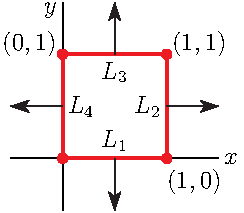
\includegraphics{OE11D_4.pdf}
\end{center}

The parametrization of $L_1$ by arc length is $\vr(s) = s\,\hi$, $0\le s\le 1$.
As the outward pointing normal to $L_1$ is $-\hj$,
\begin{align*}
\int_{L_1} \vF \cdot\hn\, \dee{s}
=\int_0^1 \vF(s,0) \cdot(-\hj)\, \dee{s}
=\int_0^1 (-0)\, \dee{s}
=0
\end{align*}
The parametrization of $L_2$ by arc length is $\vr(s) = \hi+s\,\hj$, 
$0\le s\le 1$. As the outward pointing normal to $L_2$ is $\hi$,
\begin{align*}
\int_{L_2} \vF \cdot\hn\, \dee{s}
=\int_0^1 \vF(1,s) \cdot \hi\, \dee{s}
=\int_0^1 2\, \dee{s}
=2
\end{align*}
The parametrization of $L_3$ by arc length (starting at $(1,1)$)
is $\vr(s) = (1-s)\,\hi+\hj$, $0\le s\le 1$.
As the outward pointing normal to $L_3$ is $\hj$,
\begin{align*}
\int_{L_3} \vF \cdot\hn\, \dee{s}
=\int_0^1 \vF(1-s,1) \cdot\hj\, \dee{s}
=\int_0^1 e^{1-s}\, \dee{s}
=\Big[-e^{1-s}\Big]_0^1
=e-1
\end{align*}
The parametrization of $L_4$ by arc length (starting at $(0,1)$)
is $\vr(s) = (1-s)\,\hj$,  $0\le s\le 1$. As the outward pointing 
normal to $L_4$ is $-\hi$,
\begin{align*}
\int_{L_2} \vF \cdot\hn\, \dee{s}
=\int_0^1 \vF(0,1-s) \cdot(- \hi)\, \dee{s}
=\int_0^1 (-0)\, \dee{s}
=0
\end{align*}
All together
\begin{align*}
\int_C \vF \cdot\hn\, \dee{s}
&= \int_{L_1} \vF \cdot\hn\, \dee{s}
   +\int_{L_2} \vF \cdot\hn\, \dee{s} %\\&\hskip1in
   +\int_{L_3} \vF \cdot\hn\, \dee{s}
   +\int_{L_4} \vF \cdot\hn\, \dee{s}  \\
&= 0+2+(e-1) +0 
=e+1
\end{align*}


%\noindent (b) Solution 2.\ \ 
%Alternatively, using the two dimensional variant of the divergence theorem,
% M227 PS9  or
% M317 PS8
%\begin{align*}
%\int_C \vF \cdot\hn\, \dee{s}
%&=\int_0^1\dee{x} \int_0^1\dee{y}\ \vnabla \cdot\vF(x,y)
%=\int_0^1\dee{x} \int_0^1\dee{y}\ (4x+e^x)
%=\int_0^1\dee{x} \ (4x+e^x) \\
%&=\Big[2x^2+e^x\big]_0^1 
%= e+1
%\end{align*}

\end{solution}

%%%%%%%%%%%%%%%%%%%%%%%%%%%
\begin{question}[M317 2009A] %2
A particle of mass $m = 1$ has position $\vr_0 = \hj$ and velocity 
$\vv_0 = \hi + \hk$ at time $t = 0$. The particle moves under a force
$\vF(t) = \hj - \sin t\, \hk$, where $t$ denotes time.

\begin{enumerate}[(a)]
\item
Find the position $\vr(t)$ of the particle as a function of $t$.
\item
Find the position $\vr_1$ of the particle when it crosses the plane 
$x = \pi/2$ for the first time after time $t = 0$.
\item
Determine the work done by $\vF$ in moving the particle from $\vr_0$ to 
$\vr_1$.
\end{enumerate}
\end{question}

\begin{hint} 
Force is mass times acceleration, where acceleration is the second derivative of position, $\vr(t)$, with respect to time, $t$. The work done by $\vF$ between time $a$ and time $b$
is $\int_a^b \vF\cdot\dee{\vr}$.
\end{hint}

\begin{answer} 
(a) $\vr(t) = t\,\hi+\big(1+\frac{t^2}{2}\big)\,\hj +\sin t\,\hk$\qquad
(b) $\vr_1 = \frac{\pi}{2}\,\hi+\big(1+\frac{\pi^2}{8}\big)\,\hj + \hk$
\qquad
(c) $\frac{\pi^2}{8}-\frac{1}{2}$
\end{answer}

\begin{solution} (a) Since $m=1$, Newton's law of motion gives
\begin{align*}
\va(t) = \vv'(t) = \vF(t) = \hj - \sin t\, \hk
\end{align*}
Integating gives
\begin{equation*}
\vv(t) = t\,\hj +\cos t\,\hk +\vc
\end{equation*}
for some constant vector $\vc$. Since $\vv(0)=\hi+\hk$, we have $\vc = \hi$
so that
\begin{align*}
\vr'(t) = \vv(t) = \hi + t\,\hj +\cos t\,\hk
\end{align*}
Integating again gives
\begin{equation*}
\vr(t) = t\,\hi+\frac{t^2}{2}\,\hj +\sin t\,\hk +\vc
\end{equation*}
for some (new) constant vector $\vc$. Since $\vr(0)=\hj$, we have 
$\vc = \hj$
so that
\begin{align*}
\vr(t) = t\,\hi+\left(1+\frac{t^2}{2}\right)\,\hj +\sin t\,\hk
\end{align*}

\noindent (b) The particle has $x=\pi/2$ when $t=\pi/2$ and then
\begin{align*}
\vr_1=\vr(\pi/2) = \frac{\pi}{2}\,\hi+\left(1+\frac{\pi^2}{8}\right)\,\hj + \hk
\end{align*}

\noindent (c)
The work done between time $t=0$ and time $t=\pi/2$ is
\begin{align*}
\int_0^{\pi/2} \vF(t)\cdot \dee{\vr}
&=\int_0^{\pi/2} \vF(t)\cdot \diff{\vr}{t}(t)\,\dee{t}
=\int_0^{\pi/2} [\hj-\sin t\,\hk]\cdot [\hi+t\,\hj+\cos t\,\hk]\,\dee{t} \\
&= \int_0^{\pi/2} [t -\sin t\cos t]\,\dee{t}
=\Big[\frac{t^2}{2}+\frac{1}{2}\cos^2 t\Big]_0^{\pi/2}
=\frac{\pi^2}{8}-\frac{1}{2}
\end{align*}

\end{solution}



%%%%%%%%%%%%%%%%%%%
\Instructions{Questions~\ref{path1} and \ref{path2} ask you to find a path that leads to a particular value of a line integral. Many such paths are possible --- you only need to find one.}
%%%%%%%%%%%%%%%%%%%

\begin{question}[M317 2012D]\label{path1} %3
	
	\begin{enumerate}[(a)]
		\item
		Consider the vector field $\vF\big(x,y\big)= (3y, x-1)$ in $\bbbr^2$ . Compute 
		the line integral
		\begin{equation*}
		\int_L \vF\cdot\dee{\vr} 
		\end{equation*}
		where $L$ is the line segment from $(2, 2)$ to $(1, 1)$.
		\item
		Find an oriented path $C$ from $(2, 2)$ to $(1, 1)$ such that
		\begin{equation*}
		\int_C \vF\cdot\dee{\vr} =4
		\end{equation*}
		where $\vF$ is the vector field from (a).
	\end{enumerate}
\end{question}

\begin{hint} 
	Note that the curve goes from $(2,2)$ to $(1,1)$ --- not the other way around.
	
	For part (b), one possibility is to look for a path
	consisting of the line segment from $(2,2)$ to $(2,Y)$, followed by 
	the line segment from $(2,Y)$ to $(1,Y)$, followed by the line 
	segment from $(1,Y)$ to $(1,1)$, with $Y$ being a parameter to be determined.
\end{hint}

\begin{answer} 
	(a) -5
	
	(b) One possibility is the path consisting of the line
	segment from $(2,2)$ to $(2,-3)$, followed by the line segment from
	$(2,-3)$ to $(1,-3)$, followed by the line segment from $(1,-3)$ to $(1,1)$.
	
	Another possibility is the path from $(2,2)$ to $(1,1)$ along the parabola $27x^2-80x+54$.
\end{answer}

\begin{solution} (a)
	We can parametrize $L$ by
	\begin{equation*}
	\vr(t)  = \big(x(t),y(t)\big)
	=(t,t),
	\end{equation*}
	with $t$ running from 2 to 1.
	Using this parametrization,
	\begin{align*}
	\int_L \vF\cdot\dee{\vr}
	&=\int_2^1 \vF\big(x(t),y(t)\big)\cdot(x'(t),y'(t))\ \dee{t}
	=\int_2^1 \big(3t\,,\,t-1\big)\cdot\big(1,1\big)\ \dee{t}
	\\&=\int_2^1 (4t-1)\ \dee{t} =-5
	\end{align*}
	
	\noindent (b)
	First, we note that such a choice of path is even possible: if $\vF$ were conservative, then $\int_c\vF\cdot \dee{\vr}$ would be $-5$ for every path starting at $(2,2)$ and ending at $(1,1)$, because it would be path independent. Since $\frac{\partial F_1}{\partial y}=3$ and $\frac{\partial F_2}{\partial x}=1\neq\frac{\partial F_1}{\partial y}$, by Theorem~\eref{CLP317}{thm:pathIndepConserv}, $\vF$ is \emph{not} path-independent.
	
	\textbf{Solution 1:} 
	\begin{center}
		\begin{tikzpicture}[scale=1.25]
		\YEaaxis{.5}{3}{1}{3}
		\draw (2,2) node[vertex,label=above:{$(2,2)$}](A){};
		\draw (1,1) node[vertex, label=above left:{$(1,1)$}](B){};
		\draw[ultra thick, red,->](A)--(1.5,1.5);
		\draw[ultra thick, red] (1.5,1.5)--(B);
		\draw[red] (1.3,1.75) node{$L$};
		\draw (2,-1) node[vertex,label=below right:{$(2,Y)$}](C){};
		\draw (1,-1) node[vertex, label=below left:{$(1,Y)$}](D){};
		\draw[ultra thick, blue,->] (A)--(2,1);
		\draw[ultra thick, blue, ->](2,1)--(C)--(1.5,-1);
		\draw[ultra thick, blue, ->](1.5,-1)--(D)--(1,-.5);
		\draw[ultra thick, blue,](1,-.5)--(B);
		\draw[blue] (2.25,1) node{$L_1$};
		\draw[blue] (1.5,-1.5) node{$L_2$};
		\draw[blue] (.75,.25) node{$L_3$};
		\end{tikzpicture}
		%       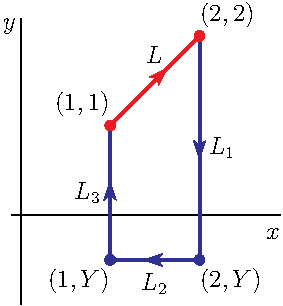
\includegraphics{OE12D_3.pdf}%arrow points in wrong direction for L
	\end{center}
	
	Let's try a family of polygonal paths $C_Y$ that consist of
	\begin{itemize}\itemsep1pt \parskip0pt \parsep0pt %\itemindent-15pt
		\item[$\circ$]
		the line segment $L_1$ from $(2,2)$ to $(2,Y)$ followed by
		\item[$\circ$]
		the line segment $L_2$ from $(2,Y)$ to $(1,Y)$ followed by
		\item[$\circ$]
		the line segment $L_3$ from $(1,Y)$ to $(1,1)$.
	\end{itemize}
	This is a way of characterizing a family of alternate paths with only one parameter, $Y$.
	We are hoping that the value of the integral
	$\int_{C_Y} \vF\cdot\dee{\vr}$ depends on $Y$ and that we can choose 
	a specific value of $Y$ so as to make the value of the integral 
	$\int_{C_Y} \vF\cdot\dee{\vr}$ exactly $4$. 
	%Just for practice, here are two separate evaluations of  
	%$\int_{C_Y} \vF\cdot\dee{\vr}$.
	
	%\emph{Direct evaluation:}\ \ \ 
	Note that
	\begin{itemize}\itemsep1pt \parskip0pt \parsep0pt %\itemindent-15pt
		\item[$\circ$]
		%We can parametrize $L_1$ as $\vr_1(t)=(2,t)$, with $t$ running from 2 to $Y$. Then $\vF(\vr_1(t))\cdot\vr_1'(t)=(3t,1)\cdot(0,1)=1$.
		On $L_1$, $x=2$ is a constant (so that $\dee{x}=0$)
		and $y$ runs from $2$ to $Y$.
		\item[$\circ$]
		%We can parametrize  $L_2$ as $\vr_2(t)=(t,Y)$ with $t$ running from 2 to 1 (and $Y$ constant).
		On $L_2$, $y=Y$ is a constant (so that $\dee{y}=0$)
		and $x$ runs from $2$ to $1$.
		%Then $\vF(\vr_2(t))\cdot\vr_2'(t)=(3Y,t-1)\cdot(1,0)=3Y$, a constant.
		\item[$\circ$]
		%We can parametrize $L_3$ as $\vr_3(t)=(1,t)$, with $t$ running from $Y$ to 1.%, 
		On $L_3$, $x=1$ is a constant (so that $\dee{x}=0$)
		and $y$ runs from $Y$ to $1$
		%Then $\vF(\vr_3(t))\cdot\vr_3'(t)=(3t,0)\cdot(0,1)=0$.
	\end{itemize}
	So,
	\begin{align*}
	\int_{C_Y} \vF\cdot\dee{\vr}
	&= \int_{L_1}\hskip-5pt \big\{(3y\,\dee{x} + (x-1)\dee{y}\big\}
	+ \int_{L_2}\hskip-5pt \big\{(3y\,\dee{x} + (x-1)\dee{y}\big\}
	+ \int_{L_3}\hskip-5pt \big\{(3y\,\dee{x} + (x-1)\dee{y}\big\} \\
	&= \int_2^Y \dee{y}
	+ \int_2^1 3Y\,\dee{x} 
	+ \int_Y^1 0\,\dee{y} \\  
	&= (Y-2) + 3Y(1-2) =-2Y-2
	\end{align*}
	
	Since we want our integral to be 4, we set $4=-2Y-2$, and find $Y=-3$. That is, the path $D$ consisting of line segments from $(2,2)$ to $(2,-3)$ to $(1,-3)$ to $(1,1)$ gives us $\int_D \vF\cdot \dee{\vr}=4$.
	
	\textbf{Solution 2:} Choosing three straight line segments was a convenient way to solve this, but not the only way. To emphasize this point, we show that we also could have considered (for example) the family of parabolas that pass through $(2,2)$ and $(1,1)$.
	
	That is, we consider the family of functions $y=ax^2+bx+c$ with $2=4a+2b+c$ and $1=a+b+c$. Subtracting the equation $a+b+c=1$ from the
equation $4a+2b+c=2$ (in order to eliminate $c$) gives
	\begin{alignat*}{6}
	&&(4a+2b+c)-(a+b+c)&=(2)-(1) \\
	 \implies&& 3a+b&=1 \\
	 \implies&& b&=1-3a
	 \intertext{Using $b=1-3a$,}
&&	a+b+c&=1 \\
	 \implies&& a+(1-3a)+c&= 1 \\ \implies&& c&=2a
	\end{alignat*}
	
	So, the class of functions described by
	$y=ax^2+(1-3a)x+2a$ for some constant $a$ are parabolas that pass through $(1,1)$ and $(2,2)$.
	
	\begin{center}
		\begin{tikzpicture}[scale=1.25]
		\YEaaxis{.5}{3}{1}{3}
		\draw (2,2) node[vertex,label=above:{$(2,2)$}](A){};
		\draw (1,1) node[vertex, label=above left:{$(1,1)$}](B){};
		\draw[ultra thick, red,->](A)--(1.5,1.5);
		\draw[ultra thick, red] (1.5,1.5)--(B);
		\draw[red] (1.3,1.75) node{$L$};
		\draw[ultra thick, blue]  plot[domain=1:1.5](\x,{3*\x*\x-8*\x+6});
		\draw[ultra thick, blue,<-]  plot[domain=1.5:2](\x,{3*\x*\x-8*\x+6});
		\draw[blue] (2,1) node[right]{$y=ax^2+(1-3a)x+2a$};
		\end{tikzpicture}
	\end{center}
	
	So, we consider paths of the form: 
	\begin{align*}
	\vr(x)&=\big(x,\ ax^2+(1-3a)x+2a\big)\\
	\vF(\vr(x))&=\big( 3ax^2+3(1-3a)x+6a,\ x-1 \big)\\
	\vr'(x)&=\big( 1,\ 2ax+1-3a\big)\\
	\vF(\vr(x))\cdot \vr'(x)&=\big(3ax^2+3(1-3a)x+6a\big)\ +\ 
	\big( 2ax^2+(1-3a)x-2ax+(3a-1)\big)\\
	&=5ax^2+(4-14a)x+(9a-1)
	\intertext{So, if $C$ is a portion of this parabola from $(2,2)$ to $(1,1)$, then}
	\int_C \vF \cdot \dee{\vr}&=\int_2^1\big(5ax^2+(4-14a)x+(9a-1)\big)\ \dee{x}\\
	&=\left[\frac{5a}{3}x^3+(2-7a)x^2+(9a-1)x\right]_2^1\\
	&=\frac{a}3-5
	\end{align*} 
	Since we want our integral to have value 4, we set $4=\frac{a}3-5$, which yields $a=27$.
	
	If we choose $C$ to be the path from $(2,2)$ to $(1,1)$ along the parabola $27x^2-80x+54$, then $\int_C\vF\cdot\dee{\vr}=4$, as desired.
\end{solution}



%%%%%%%%%%%%%%%%%%%%%%%%%%%
\begin{question}[M317 2011D] \label{path2}%6
	Let $\vF = (2y + 2)\,\hi$ be a vector field on $\bbbr^2$. Find an 
	oriented curve $C$ from $(0, 0)$ to $(2, 0)$ such that 
	$\int_C \vF\cdot \dee{\vr} = 8$.
\end{question}

\begin{hint} 
	One possibility is to look for a path
	consisting of the line segment from $(0,0)$ to $(0,Y)$, followed by 
	the line segment from $(0,Y)$ to $(2,Y)$, followed by the line 
	segment from $(2,Y)$ to $(2,0)$, with $Y$ being a parameter to be determined.
\end{hint}

\begin{answer} 
	One possibility is the path consisting of the line
	segment from $(0,0)$ to $(0,1)$, followed by the line segment from
	$(0,1)$ to $(2,1)$, followed by the line segment from $(2,1)$ to $(2,0)$.
	
	Another possibility is the path tracing out the half ellipse $\left(\cos t+1\, , \, \frac{4}{\pi}\sin t\right)$, 
	with $t$ running from $\pi$ to $0$.
\end{answer}

\begin{solution} 
	\textbf{Solution 1:}\\
	Let's try a family of polygonal paths $C_Y$ (sketched below) that consist of
	\begin{itemize}\itemsep1pt \parskip0pt \parsep0pt %\itemindent-15pt
		\item[$\circ$]
		the line segment $L_1$ from $(0,0)$ to $(0,Y)$ followed by
		\item[$\circ$]
		the line segment $L_2$ from $(0,Y)$ to $(2,Y)$ followed by
		\item[$\circ$]
		the line segment $L_3$ from $(2,Y)$ to $(2,0)$.
	\end{itemize}
	Here $Y$ is a parameter. 
	\vadjust{
		\begin{center}
			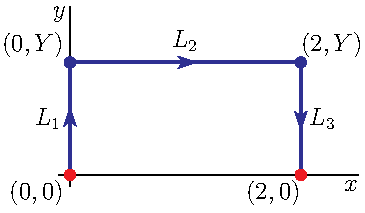
\includegraphics{OE11D_6.pdf}
		\end{center}
	}
	We are hoping that the value of the integral
	$\int_{C_Y} \vF\cdot\dee{\vr}$ depends on $Y$ and that we can choose 
	a specific value of $Y$ so as to make the value of the integral 
	$\int_{C_Y} \vF\cdot\dee{\vr}$ exactly $8$. Note that
	\begin{itemize}\itemsep1pt \parskip0pt \parsep0pt %\itemindent-15pt
		\item[$\circ$]
		on $L_1$, $x=0$ is a constant (so that $\dee{x}=0$)
		and $y$ runs from $0$ to $Y$ and 
		\item[$\circ$]
		on $L_2$, $y=Y$ is a constant (so that $\dee{y}=0$)
		and $x$ runs from $0$ to $2$ and 
		\item[$\circ$]
		on $L_3$, $x=2$ is a constant (so that $\dee{x}=0$)
		and $y$ runs from $Y$ to $0$
	\end{itemize}
	Since $\vF\cdot\dee{\vr} = (2y+2)\,\dee{x}$,
	\begin{align*}
	\int_{C_Y} \vF\cdot\dee{\vr}
	&= \int_{L_1}\hskip-5pt (2y+2)\,\dee{x}
	+ \int_{L_2}\hskip-5pt (2y+2)\,\dee{x}
	+ \int_{L_3}\hskip-5pt (2y+2)\,\dee{x} \\
	&= 0
	+ \int_0^2 (2Y+2)\,\dee{x}
	+ 0 \\  
	&= 2(2Y+2) 
	\end{align*}
	So $Y=1$ does the job.
	
	\textbf{Solution 2:}\\
	There's nothing magical about the form of the path from Solution 1. It's just a path that's relatively easy to describe using one constant $Y$. To emphasize this point, we provide a solution with an alternate path based on an ellipse.
	
	A partial ellipse running from $(0,0)$ to $(2,2)$ can be described by $\vr(t)=(\cos t+1\, , \, A\sin t)$ for a constant $A$, with $t$ running from $\pi$ to 0. (To find this: we centre a circle of radius 1 at the point $(1,0)$, then multiply its $y$-coordinate by $A$.)
	
	\begin{center}
		\begin{tikzpicture}
		\YEaaxis{.5}{4.5}{.5}{2}
		\YEycoord{1}{$A$}
		\draw (0,0) node[vertex]{};
		\draw (4,0) node[vertex, label=below:{$(2,0)$}]{};
		\draw[ultra thick, red] plot[smooth,domain=0:3.14]({2*cos(\x r)+2},{sin(\x r)});
		\end{tikzpicture}
	\end{center}
	
	In this case, $\vF(\vr(t))=(2A\sin t + 2,0)$ and $\vr'(t)=(-\sin t , A\cos t)$, so 
	\begin{align*}
	\vF(\vr(t))\cdot\vr'(t)&=-\sin t (2A\sin 2 +2)=-A(2\sin^2t)-2\sin t=-A(1-\cos2t)-2\sin t\\
	\int \vF \cdot \dee\vr&=\int_{\pi}^0\big( A(\cos2t-1)-2\sin t \big)\dee{t}=\left[A\left(\frac12\sin(2t)-t\right) +2\cos t\right]_{\pi}^0\\
	&=A\pi+4
	\end{align*}
	Setting $A\pi+4=8$, we find $A=\frac{4}{\pi}$. So, the half-ellipse $\vr(t)=\left(\cos t+1\, , \, \frac{4}{\pi}\sin t\right)$, with $t$ running from $\pi$ to 0, is another path that gives $\int_C \vF\cdot\dee\vr=8$.
\end{solution}

%%%%%%%%%%%%%%%%%%%%%%%%%%%%%%%%%%%%%%%%%%
\begin{question}[M317 2010D]  %8
Let
\begin{equation*}
\vF(x, y) = \big(1, y g(y)\big)
\end{equation*}
and suppose that $g(y)$ is a function defined everywhere with 
everywhere continuous partials.
Show that for any curve $C$ whose endpoints $P$ and $Q$ lie on the $x$-axis,
\begin{equation*}
\text{distance between $P$ and $Q$} =  \left|\int_C\vF\cdot\dee{\vr}\right|
\end{equation*}
\end{question}

\begin{hint} 
Is $\vF$ conservative?
\end{hint}

\begin{answer} 
See the solution.
\end{answer}

\begin{solution} 
The vector field $\vF$ is conservative, with 
\begin{equation*}
\vF=\vnabla\varphi\qquad
\varphi(x,y) = x+ \int_0^y \tilde y g(\tilde y)\ \dee{\tilde y}
\end{equation*}
Consquently, for $P=(x_0,0)$ and $Q=(x_1,0)$,
\begin{align*}
\int_C\vF\cdot\dee{\vr}
&=\varphi(Q)-\varphi(P)
=x_1 + \int_0^{0} \tilde y g(\tilde y)\ \dee{\tilde y}
- x_0 - \int_0^{0} \tilde y g(\tilde y)\ \dee{\tilde y} \\
&=x_1-x_0
\end{align*}
Thus
\begin{equation*}
 \left|\int_C\vF\cdot\dee{\vr}\right|
=|x(Q)-x(P)|
= \text{distance between $P$ and $Q$}
\end{equation*}

\end{solution}
%%%%%%%%%%%%%%%%%%%%%%%%%%%
\begin{question}[M317 2010A] %7
Let $S$ be the surface $z = 2 + x^2 - 3 y^2$ and let
$\vF(x , y , z) = ( xz + axy^2 )\hi + yz\hj + z^2\hk$.
Consider the points $P_1 = ( 1 , 1 , 0 )$ and $P_2 = ( 0 , 0 , 2 )$ 
on the surface $S$. 

Find a value of the constant $a$ so that
$\int_{C_1} \vF \cdot \dee{\vr}= \int_{C_2} \vF \cdot \dee{\vr}$
for any two curves $C_1$ and $C_2$ on the surface $S$ from $P_1$ to $P_2$.
\end{question}

\begin{hint} 
On $S$, note
$z = 2 + x^2 - 3 y^2$. Further, the vector field $\tilde\vF(x,y,z) = z^2\,\hk$ is 
conservative (with potential $\frac{1}{3} z^3$), so 
$\int_{C_1} \tilde\vF \cdot \dee{\vr}= \int_{C_2} \tilde\vF \cdot \dee{\vr}$
for any two curves $C_1$ and $C_2$ from $P_1$ to $P_2$. Compare this to Questions~\ref{nonconserv1} through \ref{nonconserv2}.
\end{hint}

\begin{answer} 
$a=4$
\end{answer}

\begin{solution} 
\begin{itemize}\itemsep1pt \parskip0pt \parsep0pt %\itemindent-15pt
\item[$\circ$]
First notice that the vector field $\tilde\vF(x,y,z) = z^2\,\hk$ is 
conservative (with potential $\frac{1}{3} z^3$), so 
$\int_{C_1} \tilde\vF \cdot \dee{\vr}= \int_{C_2} \tilde\vF \cdot \dee{\vr}$
for any two curves $C_1$ and $C_2$ from $P_1$ to $P_2$ (whether or not they are on the surface $S$). Consequently, the statement
``$\int_{C_1} \vF \cdot \dee{\vr}= \int_{C_2} \vF \cdot \dee{\vr}$''
is true  if and only if the statement
``$\int_{C_1} (\vF-\tilde\vF) \cdot \dee{\vr}= \int_{C_2} (\vF-\tilde\vF) \cdot \dee{\vr}$'' is true.
So we may replace the vector field $\vF$
with the vector field 
\begin{equation*}
\vG(x,y,z)=\vF(x,y,z)-\tilde\vF(x,y,z)=( xz + axy^2 )\hi + yz\hj
\end{equation*}
\item[$\circ$]
We are to consider only curves on the surface $S$.
For any such curve $C$, say parametrized by $\vr(t)$ with $a\le t\le b$, the
integral 
\begin{equation*}
\int_C \vG \cdot \dee{\vr}
=\int_a^b \vG\big(\vr(t)\big)\cdot \diff{\vr}{t}(t)\ \dee{t}
\end{equation*} 
depends only on the values of $\vG$ on the surface $S$. 
In particular, if another vector field $\vH$ obeys $\vH(x,y,z)=\vG(x,y,z)$,
for all points $(x,y,z)$ on $S$, we have
\begin{align*}
\int_C \vG \cdot \dee{\vr}
=\int_a^b \vG\big(\vr(t)\big)\cdot \diff{\vr}{t}(t)\ \dee{t}
=\int_a^b \vH\big(\vr(t)\big)\cdot \diff{\vr}{t}(t)\ \dee{t}
=\int_C \vH \cdot \dee{\vr}
\end{align*}
So we may replace $\vG$ with
\begin{align*}
\vH(x,y,z) &= \vG(x,y,2+x^2-3y^2)
  = \big[x(2+x^2-3y^2) +axy^2\big]\hi +y(2+x^2-3y^2)\hj  \\
  &= (2x+x^3 -3xy^2 +axy^2)\hi +(2y+yx^2-3y^3)\hj
\end{align*}
Note that $\vH(x,y,z)$ is defined on all of $\bbbr^3$. It just happens
to not depend on $z$.

\item[$\circ$] The curl of $\vH$ is
\begin{align*}
\vnabla\times\vH
&=\det\left[\begin{matrix}
\hi &\hj &\hk \\
\pdiff{}{x} & \pdiff{}{y} & 
                \pdiff{}{z} \\
2x+x^3 -3xy^2 +axy^2 & 2y+yx^2-3y^3 & 0
\end{matrix}
\right] \\
&=\big(2xy -[-6xy +2axy]\big)\hk
=(8-2a)xy\,\hk
\end{align*}
This is zero if $a=4$. As $\vH$ has continuous first order partial derivatives on all of $\bbbr^3$, Theorem \eref{CLP317}{thm:screenConserv} of the CLP-4 text tells us that, when $a=4$, $\vH$ is conservative and that
$\int_{C_1} \vH \cdot \dee{\vr}= \int_{C_2} \vH \cdot \dee{\vr}$
for any two curves $C_1$ and $C_2$ from $P_1$ to $P_2$
\end{itemize} 
So $a=4$ does the job.

\end{solution}

%%%%%%%%%%%%%%%%%%%%%%%%%%%
\begin{question}[M317 2009A] %3
Consider the vector field $\vF$ defined as
\begin{equation*}
\vF(x,y,z) = \Big( (1 + ax^2 )ye^{3x^2} -  bxz \cos(x^2 z)\,,\,
                    xe^{3x^2} \,,\,
                    x^2 \cos(x^2 z) \Big)
\end{equation*}
where $a$ and $b$ are real valued constants.
\begin{enumerate}[(a)]
\item
Compute $\vnabla\times\vF$.
\item
Determine for which values $a$ and $b$ the vector field $\vF$ is conservative.
\item
For the values of $a$ and $b$ obtained in part (b), find a potential function 
$f$ such that $\vnabla f = \vF$.
\item
Evaluate the line integral
\begin{equation*}
\int_C \Big(ye^{3x^2} + 2xz\cos(x^2 z)\Big) \dee{x} 
          + xe^{3x^2} \dee{y}
          + x^2 \cos(x^2 z) \dee{z}
\end{equation*}
where $C$ is the arc of the curve $(t, t, t^3)$ starting at the point 
$(0, 0, 0)$ and ending at the point $(1, 1, 1)$.

\end{enumerate}
\end{question}

\begin{hint} 
Simplify the answer in part (a) as much as possible.

For part (c), start with $\pdiff{f}{y} = xe^{3x^2}$
and $\pdiff{f}{z} = x^2 \cos(x^2 z) $.

For part (d), notice the difference between the given vector field 
and the conservative vector field of part (c). The resulting integral can be directly evaluated using methods from integral calculus.
\end{hint}

\begin{answer} 
(a) $\vnabla\times\vF
    = [-(b+2)x\cos(x^2 z)+(b+2)x^3z\sin(x^2 z)]\,\hj 
           + (6-a)x^2e^{3x^2}\,\hk $

(b) $a=6$, $b=-2$\qquad
(c) $f(x,y,z) = xye^{3x^2} +\sin(x^2 z) + C$   for any constant $C$

(d) $\frac{1}{3} e^3 +\sin 1 -\frac{1}{3}$
\end{answer}

\begin{solution} (a) The curl of $\vF$ is
\begin{align*}
\vnabla\times\vF
&=\det\left[\begin{matrix}
\hi &\hj &\hk \\
\pdiff{}{x} & \pdiff{}{y} & 
                \pdiff{}{z} \\
(1 + ax^2 )ye^{3x^2} -  bxz \cos(x^2 z) & xe^{3x^2} & x^2 \cos(x^2 z) 
\end{matrix}
\right] \\
&= 0\,\hi +[-bx\cos(x^2 z)+bx^3z\sin(x^2 z) 
            -2x\cos(x^2 z) +2x^3z\sin(x^2 z)]\,\hj \\
&\hskip1in + [e^{3x^2} +6x^2e^{3x^2}-(1 + ax^2 )e^{3x^2}]\,\hk \\
&= [-(b+2)x\cos(x^2 z)+(b+2)x^3z\sin(x^2 z)]\,\hj 
           + (6-a)x^2e^{3x^2}\,\hk 
\end{align*}

\noindent (b) For $\vF$ to be conservative it is necessary that 
$\vnabla\times\vF=\vZero$. This is the case when $b=-2$ and $a=6$.

\noindent (c) For $f$ to be a potential, when $b=-2$ and $a=6$, we need
\begin{align*}
\pdiff{f}{x}(x,y,z) 
            &= (1 + 6x^2 )ye^{3x^2} + 2xz \cos(x^2 z) \\
\pdiff{f}{y}(x,y,z) &= xe^{3x^2} \\
\pdiff{f}{z}(x,y,z) &= x^2 \cos(x^2 z)
\end{align*}
Integrating the second of these equations gives
\begin{equation*}
f(x,y,z) = xye^{3x^2} +g(x,z)
\end{equation*}
Substituting this into the last equation gives 
\begin{equation*}
\frac{\partial g}{\partial z}(x,z) = x^2 \cos(x^2 z)
\end{equation*}
which integrates to
\begin{equation*}
g(x,z) = \sin(x^2 z) + h(x)
\end{equation*}
Finally, substituting $f(x,y,z) = xye^{3x^2} +\sin(x^2 z) + h(x)$
into the first equation gives
\begin{equation*}
(1+6x^2)ye^{3x^2} +2xz\cos(x^2 z) + h'(x)
=(1 + 6x^2 )ye^{3x^2} + 2xz \cos(x^2 z)\quad\text{or}\quad
h'(x) = 0
\end{equation*}
So $h(x) = C$ and hence $f(x,y,z) = xye^{3x^2} +\sin(x^2 z) + C$  
works for any constant $C$.

\noindent (d) 
Note that the integral is 
  $\int_C\big(\vF_{a=6,b=-2}-6x^2ye^{3x^2}\hi\big)\cdot\dee{\vr}$.
So
\begin{align*}
&\int_C \Big(ye^{3x^2} + 2xz\cos(x^2 z)\Big) \dee{x} 
          + xe^{3x^2} \dee{y}
          + x^2 \cos(x^2 z) \dee{z}
 = \int_C \vnabla f\cdot\dee{\vr} -6\int_Cx^2ye^{3x^2}\,\dee{x} \\
&\hskip1in= f(1,1,1) -f(0,0,0) -6\int_0^1 t^3e^{3t^2}\,\dee{t} \\
&\hskip1in= e^3 +\sin 1 -\frac{1}{3}\int_0^3 ue^u\,\dee{u}\qquad
\text{with }u=3t^2,\ \dee{u} = 6t\,\dee{t} \\
&\hskip1in= e^3 +\sin 1 -\frac{1}{3}\Big[ue^u-e^u\Big]_0^3\qquad\text{integration by parts} \\
&\hskip1in= \frac{1}{3} e^3 +\sin 1 -\frac{1}{3}
\end{align*}


\end{solution}


%%%%%%%%%%%%%%%%%%%%%%%%%%%
%field lines are optional
%\begin{question}[M317 2001D] %2
%Let $\varphi(x,y) = xy$ and let $\vF=\nabla \varphi$.
%\begin{enumerate}[(a)]
%\item
%Find an equation for the field line of $\vF$ that passes
%through the point $(3,2)$. Sketch it and verify that it also passes through
%$(3,-2)$.
%\item
%Find $\int_{(3,-2)}^{(3,2)}\vF\cdot \dee{\vr}$, where the line integral
%is along the field line of (a).
%\end{enumerate}
%\end{question}

%\begin{hint} 
%\end{hint}

%\begin{answer}
%(a) $x=\sqrt{y^2+5}$

%\begin{center}
%   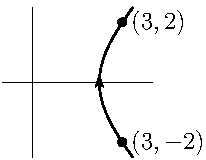
\includegraphics{OE01DQ2.pdf}
%\end{center}

%(b) $12$
%\end{answer}

%\begin{solution} 
%(a) The vector field is $\vF=\nabla\varphi = y\,\hi+x\hj$.
%All field lines have $(\dee{x},\dee{y})\parallel \vF$ so that
%$$
%\frac{\dee{x}}{y}=\frac{\dee{y}}{x}
%\iff x\,\dee{x}=y\,\dee{y}
%\iff \frac{x^2}{2}=\frac{y^2}{2}+C
%$$
%To pass through $(3,2)$, the constant $C$ must obey $\frac{3^2}{2}=\frac{2^2}{2}+C$
%or $C=\frac{5}{2}$. So the equation of the desired field line 
%is $x^2=y^2+5$. This is a hyperbola with 
%asympototes $x=\pm y$. We want the branch of the hyperbola containing
%$(3,2)$, which is $x=\sqrt{y^2+5}$. That is the branch in the sketch below. 
%The point $(-3,2)$ also obeys the equation of the hyperbola and is on 
%the same branch.

%\begin{center}
%   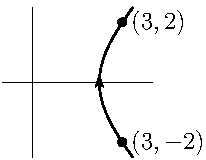
\includegraphics{OE01DQ2.pdf}
%\end{center}

%(b) Since $F$ is conservative with potential $\varphi$,
%$$
%\int_{(3,-2)}^{(3,2)}\vF\cdot \dee{\vr} = \varphi(3,2)-\varphi(3,-2)
%=3\times 2-3\times(-2)=12
%$$
%\end{solution}

%%%%%%%%%%%%%%%%%%%%%%%%%%%
\begin{question}[M317 2001A] %2
Let $C$ be the curve from $(0,0,0)$ to $(1,1,1)$ along the 
intersection of the surfaces $y=x^2$ and $z=x^3$.

\begin{enumerate}[(a)]
\item
Find $\int_C \vF\cdot \dee{\vr}$ if
 $\vF=(xz-y)\,\hi + (z+x)\,\hj+ y\,\hk$.

\item
Find $\int_C \rho\, \dee{s}$ if $s$ is arc length along $C$ and $\rho(x,y,z)=8x+36z$.

\item
Find $\int_C \vF\cdot \dee{\vr}$ if
 $\vF=\sin y\,\hi + (x\cos y+z)\,\hj+ (y+z)\,\hk$.

\end{enumerate}
\end{question}

\begin{hint} 
For (b), remember $\diff{s}{t}=\left| \diff{\vr}{t}\right|$\\
Is the vector field of part (c) conservative?
\end{hint}

\begin{answer}
(a) $\frac{23}{15} = 1.5\dot 3$\qquad
(b) $\frac{2}{3}\big[14^{3/2}-1\big]\approx 34.26$\qquad
(c) $\sin 1+\frac{3}{2} \approx 2.3415$
\end{answer}

\begin{solution} (a)
 Parametrize $C$ by $x$. Then
\begin{align*}
\vr(x)&=x\,\hi+x^2\,\hj+x^3\,\hk\qquad 0\le x\le 1\\
\vr'(x)&=\hi+2x\,\hj+3x^2\,\hk\\
\vF\big(\vr(x)\big)\cdot\vr'(x)
&=\big((x^4-x^2)\,\hi +(x+x^3)\,\hj+x^2\,\hk\big)\cdot
\big(\hi+2x\,\hj+3x^2\,\hk\big) \\
&=x^4-x^2+2x^2+2x^4+3x^4
=x^2+6x^4\\
\int_C\vF\cdot \dee{\vr}
&=\int_0^1 \big[x^2+6x^4\big]\,\dee{x}
=\Big[\frac{x^3}{3}+\frac{6x^5}{5}\Big]_0^1
=\frac{23}{15} = 1.5\dot 3
\end{align*}

(b)
 Parametrize $C$ by $x$ as in part (a). Then
\begin{align*}
\diff{s}{x}&=\left|\diff{\vr}{x}\right|=\sqrt{1+4x^2+9x^4}\\
\rho(x,x^2,x^3)\ \diff{s}{x}
&=\big(8x+36x^3\big)\sqrt{1+4x^2+9x^4}\\
\int_C\rho\ \dee{s}
&=\int_0^1 \big(8x+36x^3\big)\sqrt{1+4x^2+9x^4}\,\dee{x} 
\intertext{Using the substitution $u=1+4x^2+9x^4$, $\dee{u} = (8x+36x^3)\,\dee{x}$:}
&=\frac{2}{3}\big[1+4x^2+9x^4\big]^{3/2}\Big|_0^1\\
&=\frac{2}{3}\big[14^{3/2}-1\big]\approx 34.26
\end{align*}

(c) Since $\vF=\vnabla f$ with $f=x\sin y+yz+\frac{1}{2} z^2$,
$$
\int_C \vF\cdot \dee{\vr}=f(1,1,1)-f(0,0,0)
=\sin 1+\frac{3}{2} \approx 2.3415
$$
The potential $f$ was just guessed. Alternatively, it can be found 
by antidifferentiating:
\begin{align*}
\pdiff{f}{x}(x,y,z) 
            &= \sin y &\implies f(x,y,z)&=x\sin y + \psi_1(y,z)\\
\pdiff{f}{y}(x,y,z) &= x\cos y+z &\implies f(x,y,z)&=x\sin y+yz+\psi_2(x,z)\\
\pdiff{f}{z}(x,y,z) &= y+z&\implies f(x,y,z)&=yz+\frac12z^2+\psi_3(x,y)
\end{align*}
All together, 
$f(x,y,z) = x\sin y + yz + \frac{z^2}{2}+C$  works for any constant $C$.
\end{solution}

%%%%%%%%%%%%%%%%%%%%%%%%%%%
\begin{question}[M317 2000A] %2
 The vector field 
$\vF(x,y,z)= Ax^3y^2z\,\hi+\big(z^3+Bx^4yz\big)\,\hj
+\big(3yz^2-x^4y^2\big)\,\hk$ is conservative on $\bbbr^3$.
\begin{enumerate}[(a)]
\item
Find the values of the constants $A$ and $B$.
\item
Find a potential $\varphi$ such that $\vF=\vnabla\varphi$ on
$\bbbr^3$.
\item
If $\cC$ is the curve $y=-x,\ z=x^2$ from $(0,0,0)$ to $(1,-1,1)$,
evaluate $I=\int_\cC \vF\cdot \dee{\vr}$.
\item
Evaluate 
$J=\int_\cC (z-4x^3y^2z)\dee{x}+(z^3-x^4yz)\dee{y}+(3yz^2-x^4y^2)\dee{z}$,
where $\cC$ is the curve of part (c).
\item
Let $\cT$ be the closed triangular path with vertices $(1,0,0)$,
$(0,1,0)$ and $(0,0,1)$, oriented counterclockwise as seen from the point
$(1,1,1)$. Evaluate $\int_\cT(z\hi+\vF)\cdot \dee{\vr}$.
\end{enumerate}
\end{question}

\begin{hint} 
For part (d), what is the difference between $J$ 
and $\int_\cC\vF\cdot\dee{\vr}$?\\
For part (e), many parts of the integral are zero: find as many as you can.
\end{hint}

\begin{answer}
(a) $A=-4$, $B=-2$\qquad
(b) $\varphi(x,y,z)=-x^4y^2z+yz^3+C$
with $C$ being an arbitrary constant. \qquad
(c) $-2$\qquad
(d) $-\frac{37}{24}\approx-1.5417$\qquad
(e) $\frac{1}{2}$
\end{answer}

\begin{solution}  (a)
This field is conservative if and only if it passes the screening test 
$\vnabla\times\vF=\vZero$. That is, if and only if,
$$
\frac{\partial F_1}{\partial y}=\frac{\partial F_2}{\partial x}\qquad
\frac{\partial F_1}{\partial z}=\frac{\partial F_3}{\partial x}\qquad
\frac{\partial F_2}{\partial z}=\frac{\partial F_3}{\partial y}
$$
That is,
\begin{align*}
\frac{\partial\hfill}{\partial y}(Ax^3y^2z)
&=\frac{\partial\hfill}{\partial x}\big(z^3+Bx^4yz\big) &
&\iff &
2Ax^3yz & =4Bx^3yz
\\
%
\frac{\partial\hfill}{\partial z}(Ax^3y^2z)
&=\frac{\partial\hfill}{\partial x}\big(3yz^2-x^4y^2\big) &
&\iff &
Ax^3y^2 & =-4x^3y^2
\\
%
\frac{\partial\hfill}{\partial z}\big(z^3+Bx^4yz\big)
&=\frac{\partial\hfill}{\partial y}\big(3yz^2-x^4y^2\big) &
&\iff &
3z^2+Bx^4y& =3z^2-2x^4y
\end{align*}
Hence only $A=-4$, $B=-2$ works.

(b) When $A=-4,\ B=-2$
$$
\vF=-4x^3y^2z\,\hi+\big(z^3-2x^4yz\big)\,\hj
+\big(3yz^2-x^4y^2\big)\,\hk
%=\vnabla\big(-x^4y^2z+yz^3+C\big)
$$
We find a potential function $\varphi(x,y,z)$  for this $\vF$ by antidifferentiating.
\begin{align*}
\frac{\partial \varphi}{\partial x}(x,y,z) &= -4x^3y^2z &\implies 
\varphi(x,y,z)&= -x^4y^2z+\psi_1(y,z)\\
\frac{\partial \varphi}{\partial y}(x,y,z) &= z^3-2x^4yz &\implies \varphi(x,y,z)&=yz^3-x^4y^2z+\psi_2(x,z)\\
\frac{\partial \varphi}{\partial z}(x,y,z) &= 3yz^2-x^4y^2&\implies \varphi(x,y,z)&=yz^3-x^4y^2z+\psi_3(x,y)
\end{align*}
All together, $\varphi(x,y,z)=-x^4y^2z+yz^3+C$
with $C$ being an arbitrary constant.

(c) $I=\varphi(1,-1,1)-\varphi(0,0,0)=-2$.

(d) 
Note that $J=\int_\cC\vG\cdot\dee{\vr}$ with
\begin{align*}
\vG &= (z-4x^3y^2z)\hi+(z^3-x^4yz)\hj+(3yz^2-x^4y^2)\hk \\
    &=\vF +z\,\hi+x^4yz\,\hj
\end{align*}
so that
\begin{align*}
J%&=\int_\cC (z-4x^3y^2z)\dee{x}+(z^3-x^4yz)\dee{y}+(3yz^2-x^4y^2)\dee{z}\\
&=\int_\cC(z\hi+x^4yz\,\hj+\vF)\cdot \dee{\vr}
=-2+\int_\cC(z\hi+x^4yz\,\hj)\cdot \dee{\vr}
\end{align*}
Parametrize $\cC$ by $\vr(x)=x\,\hi-x\,\hj+x^2\,\hk$ with $0\le x\le 1$. As
$\diff{\vr}{x}=\hi-\hj+2x\,\hk$
\begin{align*}
&\int_\cC(z\hi+x^4yz\,\hj)\cdot \dee{\vr}
=\int_0^1(x^2\hi-x^7\,\hj)\cdot \big(\hi-\hj+2x\,\hk\big)\ \dee{x}
=\int_0^1(x^2+x^7)\ \dee{x}
=\frac{1}{3}+\frac{1}{8}
=\frac{11}{24} \\
&\implies J=-2+\frac{11}{24}=-\frac{37}{24}\approx-1.5417
\end{align*}

(e) 
$\cT$ is a closed path and $\vF$ is conservative, so 
$\int_\cT\vF\cdot \dee{\vr}=0$. Let $\cT_1$ be the line segment from 
$(1,0,0)$ to $(0,1,0)$,  $\cT_2$ be the line segment from 
$(0,1,0)$ to $(0,0,1)$  and $\cT_3$ be the line segment from $(0,0,1)$ to
$(1,0,0)$. 

\begin{center}
   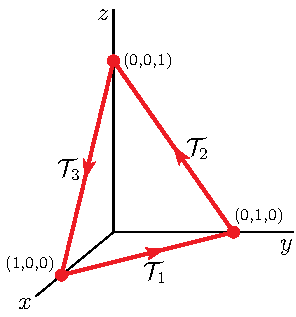
\includegraphics{OE00A_2.pdf}
\end{center}


On $\cT_1$, $z=0$, so $\int_{\cT_1}z\hi\cdot \dee{\vr}=0$. On $\cT_2$,
$x=0$, so $\hi\cdot \dee{\vr}=\dee{x}=0$ and  $\int_{\cT_2}z\hi\cdot \dee{\vr}=0$. Parametrize
$\cT_3$ by $\vr(t)=t\hi+(1-t)\hk$, $0\le t\le 1$. Then 
$\diff{\vr}{t}=\hi-\hk$ and the $z$-coordinate of the path is parametrized by $1-t$. So,
\begin{align*}
\int_\cT(z\hi+\vF)\cdot \dee{\vr}
&=\int_{\cT_3}z\hi\cdot \dee{\vr}=\int_{0}^1\overbrace{(1-t)\hi}^{z\hi}\cdot\overbrace{(\hi-\hk)\ \dee{t}}^{\dee{\vr}}\\
&=\int_0^1 (1-t) \ \dee{t}
=\frac{1}{2}
\end{align*}
 

\end{solution}

%%%%%%%%%%%%%%%%%%%%%%%%%%%%%%%
\begin{question}[M317 2017D] %3
A particle of mass
\begin{equation*}
m=2
\end{equation*}
is acted on by  a force
\begin{equation*}
\vF = \big(4t\,,\,6t^2\,,\,-4t\big)
\end{equation*}
At $t=0$, the particle has velocity zero and is located at the
point $(1,2,3)$.
\begin{enumerate}[(a)]
\item
Find the velocity vector $\vv(t)$ for $t\ge 0$.
\item
Find the position vector $\vr(t)$ for $t\ge 0$.
\item
Find $\ka(t)$ the curvature of the path traversed by the particle for $t\ge 0$.
\item
Find the work done by the force on the particle from $t=0$ to $t=T$.
\end{enumerate}
\end{question}

\begin{hint}
By Newton's law of motion, $m\vr''(t)=\vF(t)$. 

Recall $\ka(t)  = \frac{|\vr'(t)\times\vr''(t)|}{|\vr'(t)|^3}$.

\end{hint}

\begin{answer} 
(a) $\vv(t) = \big(t^2\,,\,t^3\,,\,-t^2\big) $\quad
(b) $\vr(t) 
    =\left(\frac{t^3}{3}+1\,,\,\frac{t^4}{4}+2\,,\,-\frac{t^3}{3}+3\right)$\quad
(c) $\ka(t) =\frac{\sqrt{2}}{t^2{(2+t^2)}^{3/2}}$

(d) $2T^4 + T^6$
\end{answer}

\begin{solution} 
(a) By Newton's law of motion
\begin{equation*}
m\va =\vF\quad
\implies\quad
2\vv'(t) = \big(4t\,,\,6t^2\,,\,-4t\big) \quad
\implies\quad
\vv'(t) = \big(2t\,,\,3t^2\,,\,-2t\big) 
\end{equation*}
So
\begin{equation*}
\vv(t) = \vv(0) +\int_0^t \vv'(u)\, \dee{u}
       = (0,0,0) + \int_0^t \big(2u\,,\,3u^2\,,\,-2u\big) \, \dee{u}
       = \big(t^2\,,\,t^3\,,\,-t^2\big) 
\end{equation*}

(b) From part (a), $\vr'(t) = \vv(t) = \big(t^2\,,\,t^3\,,\,-t^2\big)$.
So
\begin{align*}
\vr(t) &= \vr(0) +\int_0^t \vr'(u)\, \dee{u}
       = (1,2,3) + \int_0^t \big(u^2\,,\,u^3\,,\,-u^2\big) \, \dee{u} \\
       &= (1,2,3) + \big(t^3/3\,,\,t^4/4\,,\,-t^3/3\big)  
       =\left(\frac{t^3}{3}+1\,,\,\frac{t^4}{4}+2\,,\,-\frac{t^3}{3}+3\right)
\end{align*}

(c) From parts (a) and (b)
\begin{equation*}
|\vr'(t)|= \big|t^2(1,t,-1)\big| = t^2 \sqrt{2+t^2}
\end{equation*}
and
\begin{align*}
\vr'(t)\times\vr''(t)&= \det\left[\begin{matrix}\hi&\hj&\hk\\[0.03in] 
     t^2 & t^3 & -t^2\\
     2t  & 3t^2 & -2t\end{matrix}\right] \\
&=\big(-2t^4+3t^4\big)\,\hi -\big(-2t^3+2t^3\big)\,\hj 
          + \big(3t^4-2t^4\big)\,\hk \\
& = t^4\,\hi +t^4\,\hk \\
\implies \big|\vr'(t)\times\vr''(t)\big| &= \sqrt{2}\, t^4
\end{align*}
The curvature is (see \S\eref{CLP317}{sec:CurveCompendium} of the CLP-4 text)
\begin{align*}
\ka(t)  &= \frac{|\vr'(t)\times\vr''(t)|}{|\vr'(t)|^3}
=\frac{\sqrt{2}\, t^4}{{\big(t^2 \sqrt{2+t^2}\big)}^3} \\
&=\frac{\sqrt{2}}{t^2{(2+t^2)}^{3/2}}
\end{align*}

(d)  $W=\int \vF \cdot\dee{\vr}$:
\begin{align*}
\int_{t=0}^{t=T} \vF(t)\cdot \dee{\vr}
&=\int_0^T \vF(t)\cdot \diff{\vr}{t}(t)\,\dee{t}
=\int_0^T \big(4t\,,\,6t^2\,,\,-4t\big)\cdot 
\big(t^2\,,\,t^3\,,\,-t^2\big)\,\dee{t} \\ 
&= \int_0^T \big(8t^3+6t^5\big)\,\dee{t} 
=2T^4 + T^6
\end{align*}
\end{solution}

%%%%%%%%%%%%%%%%%%%%%%%%%%%
\begin{question}[M317 2001D] %1
	The position of an airplane at time $t$ is given by
	$
	x=y=\frac{4\sqrt{2}}{3}t^{3/2},\ z=t(2-t)
	$
	from take-off at $t=0$ to landing at $t=2$.
	\begin{enumerate}[(a)]
		\item
		What is the total distance the plane travels on this flight?
		
		\item
		Find the radius of curvature $\ka$ at the apex of the flight, which occurs
		at $t=1$.
		
		\item
		Two external forces are applied to the plane during the
		flight: the force of gravity $\vG=-M g\,\hk$, where $M$ is the mass of
		the plane and $g$ is a constant; and a friction force $\vF=-|\vv|^2\vv$,
		where $\vv$ is the velocity of the plane. Find the work done by each of
		these forces during the flight.
		
		\item
		One half-hour later, a bird follows the exact same flight --- path
		as the plane, travelling at a constant speed $v=3$. One can show that 
		at the apex of the path, i.e. when the bird is at 
		$\big(\frac{4\sqrt{2}}{3},\frac{4\sqrt{2}}{3},1\big)$, the principal
		unit normal $\hN$ to the path points in the $-\hk$ direction. Find the bird's (vector)
		acceleration at that moment. 
	\end{enumerate}
\end{question}

\begin{hint}
	(a) Remember the arclength of the parametrized path $\vr(t)$ from $t=a$ to $t=b$ is given by $\int_a^b |\vr'(t)|\ \dee{t}$. In this case, $|\vr'(t)|$ can be simplified considerably.\\
	(b) Remember $\ka(t)  = \frac{|\vr'(t)\times\vr''(t)|}{|\vr'(t)|^3}$.\\
	(c) Gravity is conservative. Friction is not conservative.\\	
	(d) What are the tangential and normal components of acceleration? 
\end{hint}

\begin{answer} 
	(a) $8$\qquad
	(b) $\frac{1}{8}$\qquad
	(c) $-\frac{16}{5}(3^5-1)\approx-774.4$\qquad
	(d) $\Big(0,0,-\frac{9}{8}\Big)$
\end{answer}

\begin{solution} (a)  
	For the specified curve
	\begin{align*}
	\vr(t)&=\Big(\frac{4\sqrt{2}}{3}t^{3/2},\frac{4\sqrt{2}}{3}t^{3/2},
	t(2-t)\Big)\\
	\vv(t)=\vr'(t)&=\big(2\sqrt{2}t^{1/2},2\sqrt{2}t^{1/2},2-2t\big)\\
	|\vv|&=\sqrt{8t+8t+4-8t+4t^2}=\sqrt{4(1+2t+t^2)}= 2|1+t|=2(1+t)
	\end{align*}
	So the distance travelled is 
	$$
	\int_0^2|\vv(t)|\,\dee{t}=\int_0^2 2(1+t)\,\dee{t} = 2\Big[t+\frac{t^2}{2}\Big]_0^2
	=8
	$$
	
	(b) As
	\begin{align*}
	\vv(t)=\vr'(t)&=\big(2\sqrt{2}t^{1/2},2\sqrt{2}t^{1/2},2-2t\big) &
	\vv(1)&=2\sqrt{2}\big(1,1,0\big)\\
	\va(t)=\vv'(t)&=\big(\sqrt{2}t^{-1/2},\sqrt{2}t^{-1/2},-2\big) &
	\va(1)&=\sqrt{2}\big(1,1,-\sqrt{2}\big)\\
	\vv(1)\times\va(1)&=4\big(-\sqrt{2},\sqrt{2},0\big) &
	|\vv(1)|&=4
	\end{align*}
	the curvature
	\begin{align*}
	\ka(1) &= \frac{|\vv(1)\times\va(1)|}{|\vv(1)|^3}
	=\frac{8}{4^3}
	=\frac{1}{8}
	\end{align*}
	
	(c) $\vG=\nabla\varphi$ with $\varphi(x,y,z)= - Mgz$, so that gravity is conservative.
	The work done is 
	$$
	\varphi\big(\vr(2)\big)-\varphi\big(\vr(0)\big)
	=\varphi\big(\nicefrac{16}{3}\,,\,\nicefrac{16}{3}\,,\,0\big)
	-\varphi(0,0,0)=0
	$$
	Friction is not conservative, so we have to compute the work long hand.
	\begin{align*}
	\int_0^2\!\! \vF\cdot \dee{\vr} 
	&=\int_0^2\!\! \vF(t)\cdot \diff{\vr}{t}(t)\,\dee{t} 
	=-\int_0^2 |\vv(t)|^2\vv(t)\cdot \vv(t)\,\dee{t} 
	=-\int_0^2 |\vv(t)|^4\,\dee{t} \\
	&=-2^4\int_0^2 (1+t)^4\,\dee{t} 
	=-\frac{16}{5}(1+t)^5\Big|_0^2\\
	&=-\frac{16}{5}(3^5-1)\approx-774.4
	\end{align*}
	
	(d)	 \textbf{Solution 1:}\qquad
	We know, from Theorem \eref{CLP317}{thm:curvatureFormulae}.c in the 
	text, that
	\begin{equation*}
	\va(t)  = \difftwo{s}{t}\hat\vT + \ka\Big(\diff{s}{t}\Big)^2\hat\vN
	\end{equation*}
	We have also been told that, at the apex, $\hat\vN=-\hk$ and 
	that $\diff{s}{t}(t)=3$ for all $t$.
	So $\difftwo{s}{t}=0$. As $\ka=\frac{1}{8}$ at the apex
	\begin{equation*}
	\va(1)  = 0\hat\vT + \frac{1}{8}\big(3\big)^2(-\hk)
	= -\frac{9}{8}\hk
	\end{equation*}
	
	\textbf{Solution 2:}
	\qquad
	The bird follows the parametrized path 
	\begin{equation*}
	\vr(u)=\left(\frac{4\sqrt{2}}{3}u^{3/2},\frac{4\sqrt{2}}{3}u^{3/2},
	u(2-u)\right)
	\end{equation*}
	This is the same path as the plane, but the parameter
	$u$ is not time. Let's denote by $\vR(t)$ the position of 
	the bird at time $t$. At time $t$ the bird is at some point on
	the parametrized path, so there is some $u(t)$ with
	\begin{equation*}
	\vR(t) = \vr\big(u(t)\big)
	\end{equation*} 
	
	We saw in part (a) that $\big|\diff{\vr}{u}\big|
	=2(1+u)$. Since the bird always has speed $3$,
	\begin{align*}
	&3=\Big|\diff{\vR}{t}(t)\Big|=\Big|\diff{\vr}{u}(u(t))\diff{u}{t}\Big|
	=2\big(1+u(t)\big)\diff{u}{t} \\
	&\implies \diff{u}{t}=\frac{3}{2(1+u(t))}
	\implies \difftwo{u}{t}=-\frac{3}{2(1+u(t))^2}\diff{u}{t}
	=-\frac{9}{4(1+u(t))^3}
	\end{align*}
	At the apex $u=1$ so that $\diff{u}{t}=\frac{3}{4}$ and 
	$\difftwo{u}{t}=-\frac{9}{32}$. The bird's acceleration is
	$$
	\difftwo{\vR}{t}(t)=\diff{}{t}\Big(\diff{\vR}{t}(t)\Big)
	=\diff{\hfill}{t}\Big(\diff{\vr}{u}(u(t))\diff{u}{t}(t)\Big)
	=\difftwo{\vr}{u}\Big(\diff{u}{t}\Big)^2
	+\diff{\vr}{u}\difftwo{u}{t}
	$$
	From part (a)
	\begin{align*}
	\diff{\vr}{u}&=\big(2\sqrt{2}u^{1/2},2\sqrt{2}u^{1/2},2-2u\big)\\
	\difftwo{\vr}{u}&=\big(\sqrt{2}u^{-1/2},\sqrt{2}u^{-1/2},-2\big)\\
	\end{align*}
	At the apex, when $u=1$,
	\begin{align*}
	\diff{\vr}{u}&=\big(2\sqrt{2},2\sqrt{2},0\big)\\
	\difftwo{\vr}{u}&=\big(\sqrt{2},\sqrt{2},-2\big)\\
	\end{align*}
	and the acceleration is
	\begin{align*}
	\difftwo{\vR}{t}
	&=\difftwo{\vr}{u}\Big(\diff{u}{t}\Big)^2
	+\diff{\vr}{u}\difftwo{u}{t}
	=\big(\sqrt{2},\sqrt{2},-2\big)\Big(\frac{3}{4}\Big)^2
	+\big(2\sqrt{2},2\sqrt{2},0\big)\Big(-\frac{9}{32}\Big) \\[0.05in]
	&=\Big(0,0,-\frac{9}{8}\Big)
	\end{align*}
\end{solution}